\documentclass[deutsch]{report}

% \usepackage[utf8]{inputenc}
% %\usepackage{url}
% \usepackage{hyperref}
% %\usepackage[T1]{fontenc}
% \usepackage[utf8]{inputenc}
% \usepackage{fontspec}

% \usepackage[default,oldstyle,scale=0.95]{opensans} %% Alternatively
% %% use the option 'defaultsans' instead of 'default' to replace the
% %% sans serif font only.
% \usepackage[T1]{fontenc}

%\setmainfont{lato}

%\renewcommand{\familydefault}{\sfdefault}

%clickable tableofcontent
\usepackage{hyperref}

%degree
\usepackage{siunitx}

\usepackage{booktabs,caption}
\usepackage[flushleft]{threeparttable}
\usepackage[T1]{fontenc}

%german support
\usepackage[ngerman]{babel}
%\usepackage[ansinew]{inputenc}

%images
\usepackage{graphicx}
\graphicspath{ {./images/Software/}{./images/Hardware/} }

%absätze
\usepackage{parskip}

%mathsections
\usepackage{amsmath}

\usepackage[backend=biber,
    style=numeric,
    autocite=plain,
    sorting=none]{biblatex}
%citestyle=authoryear]{biblatex}
\addbibresource{CitationDB.bib}



\title{Entwicklung und Untersuchungen zur Nutzbarkeit eines Rollstuhls als Eingabegerät zur Navigation im virtuellen Raum}
\author{Benedikt Christian Beigang}
\date{\parbox{\linewidth}{\centering%
        \today\endgraf\bigskip
        Fakultät Informatik und Medien \endgraf
        HTWK Leipzig}}

\begin{document}
\maketitle

\addcontentsline{toc}{chapter}{Abstract}
\chapter*{Abstract}

\tableofcontents{}

\chapter{Einleitung}
Mit dem Aufkommen von Computern entwickelten sich parallel die unterschiedlichsten Geräte und Methoden, mit denen Anweisungen an die Rechenmaschine übermitteln werden können.
Anfangs noch mit Schaltern und Lochkarten, entwickelten sich nach und nach, die unterschiedlichsten Eingabegeräte und Methoden, um den Maschinen präzise zu vermitteln, was diese tun sollen.
Das Entstehen der verschiedensten virtuellen Umgebungen führte zum Wunsch, in diesen möglichst barrierefrei zu navigieren.
So setzten sich beispielsweise Computermäuse durch, mit der Verbreitung erster Mikrocomputer mit graphischer Benutzeroberfläche.
Grund dafür ist, dass die Navigation in einer zweidimensionalen Umgebung mit ihr vereinfacht wurde.
Manche Eingabegeräte wurden aus anderen Bereichen, in die Welt des Computers übersetzt, wie zum Beispiel die Schreibmaschine hin zur Tastatur.
Ein völlig neues Design hingegen war der Spielcontroller, der durch die Entwicklung von Videospielen und Spielkonsolen hervorkam.
Dieser stellte sich nicht nur als geeignetes Eingabegerät im zweidimensionalen Raum raus, sondern auch im dreidimensionalen.

Heute erlauben eingebettete Systeme theoretisch jeden Gegenstand in ein Eingabegerät zu verwandeln.
Solange ein Gegenstand unterschiedliche Zustände abbilden kann, ist es möglich, über die Manipulation dieser Zustände dem Computer Anweisungen zu übermitteln.
Begrenzt wird die Anzahl unterschiedlicher Anweisungen nur durch die Anzahl der verschiedenen Zustände, die das Eingabegerät annehmen kann.
Jedoch muss gleichzeitig auch gewährleistet sein, dass jeder Nutzer einfach, präzise und bequem die Eingaben tätigen kann.

Ein Gegenstand, der nur vereinzelt als Eingabegerät in Betracht gezogen wurde, ist der Rollstuhl.
Durch die geringe Anzahl von Eingaben, bedingt durch die zwei Räder, ist der Nutzer eingeschränkter als bei anderen Eingabegeräten.
So kann die Frage entwickelt werden, inwieweit man sich mit einem Rollstuhl im virtuellen Raum bewegen und mit ihm interagieren kann und was nötig ist, um ein solches System zu entwickeln.
In der Vergangenheit wurde mithilfe von aufwändigen Konstruktionen Simulationen eines Rollstuhls entwickelt, welche mit einem echten Rollstuhl gesteuert werden können.
Jedoch beschränkten sich diese auf die möglichst exakte Simulation der Bewegung, inklusive Krafteinwirkung auf die Räder, wenn in der virtuellen Welt der Boden uneben ist.
Für einen privaten Nutzer, der seinen Rollstuhl als Eingabegerät an seinem Heimrechner nutzen möchte, sind die bislang entwickelten Systeme ungeeignet.

Diese Arbeit widmet sich der Frage, mit welchen Mitteln ein Rollstuhl als Eingabegerät, für den Gebrauch am Heimcomputer, umfunktioniert werden kann und wie die Bewegungen der Räder des Rollstuhls in geeignete Anweisungen für den Computer abgebildet werden können.
Möglichst viele Anwendungen sollen dabei theoretisch vom Rollstuhl gesteuert werden können.
Das System soll dabei klein und kostengünstig sein, sodass es für einen privaten Nutzer praktikabel und erschwinglich ist.
Dafür werden im Rahmen dieser Arbeit zunächst einige Begriffe erläutert, die Bachelor-Thesis im Kontext aktueller Forschung verortet, sowie anschließend ein eingebettetes System entwickelt und analysiert.
Dieses System übermittelt die Rotationsdaten der Räder an eine externe Software (im Folgenden Rollstuhl-Software genannt), die auf dem selben Betriebssystem läuft wie die zu steuernde Anwendung.
Zuletzt werden Verfahren implementiert und untersucht, mit dem die empfangenen Daten auf Eingaben eines herkömmlichen Eingabegeräts abgebildet werden können, damit die Anweisungen auch von anderer Software gelesen werden kann.
Dabei soll dem Nutzer eine möglichst hohe Bewegungs- und Interaktionsfreiheit geboten sein.
\chapter{Begriffsklärung}
Im Folgenden sollen nicht triviale Begriffe erklärt werden, die für das Verständis dieser Arbeit notwendig sind.

%------------------------------------------------------------------------------------------------------
\section{Eingebettetes System}
Ein eingebettetes System besteht aus einem programmierbaren Mikroprozessor und wird meist umgeben von Sensoren und Aktoren.
Das gesamte System bildet damit eine Schnittstelle zwischen physikalischen Prozessen und einem elektrischen Gerät.

Marwedel definiert ein eingebettetes System wie folgt:
\begin{quote}
    „Eingebettete Systeme sind informationsverarbeitende Systeme, die in umgebende Produkte integriert sind.“\cite{marwedelEingebetteteSystemeGrundlagen2021}
\end{quote}

Gessler erweitert diese Definition und schreibt:
\begin{quote}
    „Das Eingebettete Systeme sind Rechenmaschinen, die in elektrischen Geräten „eingebettet“ sind, z. B. in Kaffeemaschinen, CD-, DVD-Spielern oder Mobiltelefonen.
    Unter eingebetteten Systemen verstehen wir alle Rechensysteme außer den Desktop-Computern.“\cite{gesslerEntwicklungEingebetteterSysteme2014}
\end{quote}

Da für das Steuern von Aktoren und das Auslesen von Sensoren, sowie das Empfangen und Übertragen von Daten aus heutiger Sicht keine große Rechenleistung benötigt wird, sind die verwendeten Mikroprozessoren verglichen mit modernen Prozessoren weniger leistungsstark.
Das hat zur Folge, dass Randbedingungen entstehen, welche bei der Entwicklung beachtet werden müssen.
Dazu zählen Rechenleistung, Verlustleistung und Ressourcenverbrauch\cite{gesslerEntwicklungEingebetteterSysteme2014}.
Jedoch sind grade deshalb solche Systeme erschwinglich, da keine Hardware benötigt wird, welche auf maximale Rechenleistung und Speicherverbrauch ausgelegt ist.
Aktuell sind eingebettete Systeme in den unterschiedlichsten Anwendungsgebieten zu finden, so zum Beispiel in: Autos, Schienenfahrzeuge, Flugzeugen, in der Telekommunikation und bei der Fertigungsautomatisierung\cite{marwedelEingebetteteSystemeGrundlagen2021}.
Eingebettete Systeme werden meist mit hardwarenahen Sprachen programmiert wie C und C++, da diese durch ihre Nähe zur Hardware die höchste Effizienz versprechen\cite{gesslerEntwicklungEingebetteterSysteme2014}.

%------------------------------------------------------------------------------------------------------
\section{Virtueller Raum}
Der Begriff des Raums ist in den unterschiedlichsten Fachbereichen zu finden, mit den verschiedensten Bedeutungen.
In der Mathematik gibt es viele Arten von Räumen (algebraischer Raum, euklidischer Raum, Hilbert Raum, etc.), die präzise definiert werden können.
Kulturwissenschaftlich spielt der Raum ebenfalls eine große Rolle, jedoch nicht als mathematisches Konstrukt, sondern bezieht zwischenmenschliche und gesellschaftliche Aspekte mit ein.
Der Begriff des \textit{virtuellen Raums} ist jedoch nicht klar eingrenzbar.
Da sich die verschiedensten Fachbereiche ihm bedienen, hängt die Definition davon ab, aus welcher Richtung man sich ihm nähert.
Deshalb wird im Zuge dieser Arbeit der Begriff des \textit{virtuellen Raums} wie folgt definiert:

Ein virtueller Raum ist ein durch einen Computer erzeugte Umgebung, welche auf eine zweidimensionale Projektionsfläche abgebildet werden kann.
Es ist kein im physikalischen Sinne real existierender Raum mit messbaren Abmessungen.
Wie auch in anderen Räumen ist es auch im virtuellen Raum möglich, durch ihn hindurch zu navigieren.
So hat der Nutzer eine Position in diesem, sowie die Möglichkeit diese Position gezielt zu verändern.

In der vorliegenden Arbeit wird vorwiegend mit dreidimensionalen Räumen gearbeitet, auch wenn zweidimensionale Räume denkbar sind.
Ein Beispiel für zweidimensionale Räume ist ein \ac{gui}; der Nutzer kann innerhalb dieser zwischen verschiedenen Bereichen navigieren.
Dazu werden Hyperlinks und Steuerungselemente wie ein Knopf verwendet.
Ein Beispiel für dreidimensionale Räume sind 3D-Computerspiele.
Für diese wird ein euklidischer Raum berechnet, in dem der Spieler selbstbestimmt umherwandern kann.
Jedoch kann auch eine \ac{gui} zusätzlich mit eingebettet sein.

%------------------------------------------------------------------------------------------------------
\section{Navigation}
Der Duden definiert das Verb \textit{navigieren} wie folgt:

\begin{quote}
    1. „den Standort eines Schiffes oder Flugzeugs bestimmen und es auf dem richtigen Kurs halten“\\
    2. „(z. B. bei der Suche nach Informationen im Internet) [gezielt] ein Programm oder einen Programmpunkt nach dem anderen aktivieren“
    \cite{DudenNavigierenRechtschreibung}
\end{quote}

Ursprünglich kommt das Wort aus der Seefahrt.
Früher wurden „\textit{Landmarken, die Küste, Meeresströmungen, Lotungen der Wassertiefen, jahreszeitliche regelmäßige Winde, Wolkenansammlungen und der Flug der Zugvögel}“\cite{wolfschmidtNavigareNecesseEst2008} genutzt, um die aktuelle Position des eigenen Schiffes bestimmen zu können.
Somit konnte sichergestellt werden, dass das Schiff sein Ziel erreicht.
Im Laufe der Zeit kamen immer mehr Methoden und Werkzeuge zum Einsatz, um immer präziser die eigene Position ermitteln und den optimalen Weg bestimmen zu können.
Jedoch beschränkt sich das Wort nicht auf das Herausfinden der eigenen Position, sondern schließt die Tätigkeit der Wegfindung, sowie das Kurshalten eines vorher festgelegten Pfades mit ein.

Mit dem Aufkommen neuer Verkehrsmittel wie dem Flugzeug und Technologien wie GPS wurde der Begriff der Navigation weiter gefasst.
So definiert der Medienwissenschaftler Florian Sprenger Navigation wie folgt: „\textit{… eine Praxis des Umgangs mit Relationen.}“\cite{sprengerNavigationenUndRelationen2022}.
Das navigierende Individuum oder Objekt entscheidet auf Grundlage von „\textit{medial ver- oder kulturtechnisch ermittelten Verhältnis zu anderen Objekten […] oder durch Repräsentationen dieser Relationen auf imaginären, geographischen oder digitalen Karten}“ in welche Richtung sich bewegt werden muss\cite{sprengerNavigationenUndRelationen2022}.

Im Kontext dieser Arbeit navigiert der Nutzer auf einer zweidimensionalen Ebene, in einem dreidimensionalen virtuellen Raum.
Er steuert dabei gezielt seine Fortbewegung und interagiert mit der virtuellen Umgebung, indem die Räder eines Rollstuhls, in dem er sitzt, gedreht werden.
Es soll im Rahmen dieser Arbeit zusätzlich hervorgehoben werden, dass Navigation im Gegensatz zum reinen Fortbewegen nicht passiv ist.
Das Objekt oder Individuum, das navigiert, hat einen Einfluss auf die Richtung der Fortbewegung.

%------------------------------------------------------------------------------------------------------
\section{Gyroskop}
Ein Gyroskop ist ein Sensor, der genutzt wird, um „\textit{die Winkelgeschwindigkeit um eine feste Achse}“ zu messen\cite{armeniseAdvancesGyroscopeTechnologies2010}.
Es gibt verschiedene Arten von Gyroskopen, die Messungen mit unterschiedlichen Methoden vornehmen.
So wird zwischen drei Arten von Gyroskopen unterschieden: optische, vibrierende und welche, bei denen eine Masse rotiert.
Mithilfe von \ac{mems} konnten Trägheitssensoren miniaturisiert und in Massen produziert werden.
In der Elektrotechnik sind diese beliebt, da sie klein und kostengünstig sind\cite{maenakaMEMSInertialSensors2008}.
Sie messen die Coriolis-Kraft, welche durch die Rotation entlang von voher festgelegten Achsen wirkt.
Der Sensor kann diese Kraft messen und als elektrisches Signal weitergeben, sodass anschließend das Signal digitalisiert werden kann\cite{utmelMPU6050ModuleDatasheet}.
Heute sind sie in durch ihre Verfügbarkeit in den verschiedensten Anwendungsgebieten zu finden, wie dem Auto, der Medizin oder der Unterhaltungselektronik\cite{armeniseAdvancesGyroscopeTechnologies2010}.

%------------------------------------------------------------------------------------------------------
\section{Eingabegerät}
Im Buch \textit{Virtual und Augmented Reality (VR/AR)} von 2013 werden Eingabegeräte wie folgt beschrieben:

\begin{quote}
    „Eingabegeräte dienen der sensorischen Erfassung von Nutzerinteraktionen.“\cite{doernerVirtualUndAugmented2013}
\end{quote}

Das heißt, dass Eingabegeräte eine Schnittstelle von Mensch zu Maschine darstellen.
Jedes benötigt dazu einen Sensor der eine physikalische Zustandsveränderung, meistens eine Bewegung, in ein elektrisches Signal umwandelt.
Ein Computer kann das erzeugte Signal auslesen und interpretiert aus diesem eine auszuführende Anweisung.
Je nach Anwendungsgebiet sind unterschiedliche Eingabegeräte geeigneter.
So ist für das Schreiben eines Textes eine Tastatur nutzerfreundlicher im Vergleich zu einem Spielcontroller.
Ein Eingabegerät kann aus mehreren Eingabetypen bestehen.
Die gängigsten sind binäre und stufenlose Tasten, sowie welche entlang von Achsen, wie beispielsweise Thumbsticks oder Touchpads.
Darüber hinaus gibt es noch weitere Eingabetypen, diese zu nennen, jedoch den Rahmen ausreizen würde.
Allgemein lässt sich festhalten:
Ist ein Mensch fähig die Messwerte eines Sensors zu manipulieren, kann dieser als Eingabegerät verwendet werden kann.
\chapter{Stand der Forschung}
\chapter{Entwicklung des eingebetteten Systems}
Damit der Rollstuhl-Software bekannt ist, mit welcher Geschwindigkeit sich welches Rad in welche Richtung dreht, ist Hardware notwendig.
Um dies zu bewerkstelligen wurde ein eingebettetes System entwicklet. Dieses muss die Rotationsdaten messen und an die Software übermitteln.
Dabei kommt ein ESP32-Mikrocontroller zum Einsatz der ein Gyroskop ausliest und anschließend die Daten mithilfe eines Funkprotokolls an die Rollstuhl-Software überträgt.
Näher soll in einem Vergleich beleuchtet werden, ob WiFi und ESP-Now das geeignetere Übertragungsprotokoll ist.

\section{PlatformIO}
Zur Entwicklung der eingebetteten Software, die auf den Mikrocontrollern läuft, wurde PlatformIO verwendet.
Dies ist eine Framework-Erweiterung für Visual Studio Code, bei der die benötigten Bibliotheken, die für jeden Mikrocontroller und jedes Board notwendig sind, automatisch heruntergeladen und eingerichtet werden.
Ebenfalls lassen sich über das UI, Bibliotheken, die für das jeweilige Projekt notwendig sind, hinzufügen.
Zusätzlich zur Entwicklungsumgebung von Visual Studio Code gibt es Funktionalitäten einen Chip zu flashen und anschließend im seriellen Monitor die Ausführung zu beobachten.
Im Gegensatz zu Umgebungen wie der Arduino IDE wird Zeit gespart, da dort zunächst manuell Treiber heruntergeladen werden müssen.
Zusätzlich kann man nicht von den Vorteilen einer modernen IDE profitieren.

\section{Messung der Raddaten}
Um die Rotation der Räder des Rollstuhls messen zu können, wird ein Sensor benötigt.
Dabei wurde sich für ein Gyroskop entschieden, da diese verfügbar, kostengünstig und leicht integrierbar sind.
\footnote{warum keine lichtschranke} Jedoch erfordert die Verwendung eines Gyroskops eine Voreinstellung und Kalibrierung, welche in diesem Unterkapitel erörtert werden.

\subsection{Gyroskop}
Im Zuge dieser Arbeit habe ich mich für das Motion-Tracking-Device GY-521 MPU-6050 entschieden.
Dieses ist klein (mit Pins: 20mm x 15mm x 11mm), kostengünstig zu erwerben (ca. 4 Euro) und verfügt unter anderem über 3-Achsen-Gyroskop-Sensoren, mit denen die Rotation gemessen werden kann.
Der Chip besitzt folgende 8 Anschlüsse (S.7)\cite{GY5216AchsenGyroskop}:

\begin{table}[h]
    \centering
    \begin{threeparttable}
        \caption{Pins des GY-521 MPU-6050}
        \begin{tabular}{|l|l|l|}
            \hline
            \textbf{Anschluss}          & \textbf{Funktion}        & \textbf{Notwendig} \\ \hline
            \parbox[c][0.5cm]{2cm}{VCC} & Power-Supply             & Ja                 \\ \hline
            \parbox[c][0.5cm]{2cm}{GND} & Ground                   & Ja                 \\ \hline
            \parbox[c][0.5cm]{2cm}{SCL} & I2C Serial-Clock Line    & Ja                 \\ \hline
            \parbox[c][0.5cm]{2cm}{SDA} & I2C Serial-Date Line     & Ja                 \\ \hline
            \parbox[c][0.5cm]{2cm}{XDA} & Auxiliary Serial Data    & Nein               \\ \hline
            \parbox[c][0.5cm]{2cm}{XCL} & Auxiliary Serial Clock   & Nein               \\ \hline
            \parbox[c][0.5cm]{2cm}{ADO} & I2C Address Select       & Ja                 \\ \hline
            \parbox[c][0.5cm]{2cm}{INT} & Interrupt Digital Output & Nein               \\ \hline
        \end{tabular}
    \end{threeparttable}
\end{table}

Die Daten können mithilfe eines angeschlossenen Mikrocontrollers (ESP32) ausgelesen werden.
Jede Achse wird auf zwei 8-Bit-Register abgebildet (S. 31)\cite{MPU6000MPU6050Register2013}.
Zusammen ergibt das einen Wertebereich von 65.536 unterscheidbaren Zuständen.
Mit der Drehrichtung rückwärts halbiert sich dieser Wertebereich, da ein Bit für das Verschieben des Wertebereichs ins Negative benötigt wird.
Das Gyroskop des MPU-6050 kann in vier verschiedenen Konfigurationen betrieben werden (S. 31)\cite{MPU6000MPU6050Register2013}.
Damit wird festgelegt, wie klein der Winkel zwischen zwei verschiedenen Zuständen ist; mit anderen Worten, wie viele Stufen pro Grad unterschieden werden können.
Da der Wertebereich konstant ist, bedeutet eine empfindlichere Messung, dass das Gyroskop bei einer geringeren Geschwindigkeit das Ende des Wertebereichs erreicht.
Angewendet auf den Rollstuhl hat das zur Folge, dass das rotierende Rad bei niedrigeren Geschwindigkeiten seine maximal messbare Geschwindigkeit erreicht.

\begin{table}[h]
    \centering
    \begin{threeparttable}
        \caption{Einstellbare Modi des Gyroskops mit ihren resultierenden Eigenschaften}
        \begin{tabular}{|l|l|l|l|l|}
            \hline
            ~ & \textbf{Modus 0} & \textbf{Modus 1} & \textbf{Modus 2} & \textbf{Modus 3} \\ \hline
            \parbox[c][1cm]{4cm}{\textbf{Maximale Gradzahl                                \\pro Sekunde}}                   & 250     & 500     & 1000    & 2000    \\ \hline
            \parbox[c][1cm]{4cm}{\textbf{Stufen                                           \\pro Grad }}                                & 131     & 65,5    & 32,8    & 16,4    \\ \hline
            \parbox[c][1.5cm]{4cm}{\textbf{Maximale                                       \\Umdrehungszahl \\pro Sekunde }  }          & 0,69    & 1,39    & 2,78    & 5,56    \\ \hline
            \parbox[c][1cm]{4cm}{\textbf{Maximale Radianten                               \\pro Sekunde     }  }           & 4,36    & 8,73    & 17,47   & 34,93   \\ \hline
            \parbox[c][1.5cm]{4cm}{\textbf{Zurückgelegte Distanz                          \\pro Stufe\\in Millimetern*}} & 0,04    & 0,08    & 0,16    & 0,32    \\ \hline
        \end{tabular}
        \begin{tablenotes}
            \small
            \item Werte bei einem Raddurchmesser von 60 cm – (S. 31) \cite{MPU6000MPU6050Register2013} ergänzt um eigene Werte
        \end{tablenotes}
    \end{threeparttable}
\end{table}

Es stellt sich die Frage, welcher der optimale Modus für das hier entwickelte System ist.
Um dem Nutzer ein möglichst störungsfreies Erlebnis zu bieten, muss gewährleistet sein, dass das Gyroskop so empfindlich wie möglich eingestellt ist.
Das bedeutet, dass der Wertebereich maximal ausgereizt werden muss.
Ist der Modus nicht empfindlich genug, so bemerkt der Nutzer möglicherweise das Springen der Bitwerte in Form eines Vorspringens in der Bewegung.
Allerdings muss ein Modus gewählt werden, welcher dazu führt, dass der Nutzer nicht schneller als die maximale Gradzahl pro Sekunde drehen kann, da es sonst zu einem Zahlenüberlauf kommt und zu einer fehlerhaften Weiterverarbeitung der Daten führt.
Der Zahlenüberlauf kann zwar abgefangen werden, jedoch sollte bei Bedarf einer maximale Geschwindigkeit diese programmgesteurert festgelegt werden.
Dies birgt den Vorteil den maximalen Wert flexibler setzen zu können.
Der Modus muss also so empfindlich sein, dass der Nutzer nicht den Übergang von einem Zustand in den nächsten registriert.
Gleichzeitig darf er nicht in der Lage sein, die Räder schneller als die maximale Gradzahl pro Sekunde zu drehen.
Im Kapitel System-Analyse wird dieser Frage weiter nachgegangen.

\subsection{Verbesserung der Rohdaten}
Die ausgelesenen Werte des Gyroskops sind nicht automatisch kalibriert.
Sie besitzen einen konstanten Offset. Deshalb muss beim Start des Systems eine Kalibrierungssequenz gestartet werden.
Diese errechnet aus einer Reihe ausgelesener Werte einen Mittelwert, der anschließend von allen zukünftigen Werten abgezogen wird.
Dazu dürfen die Räder nicht bewegt werden, da dies das Ergebnis der Kalibrierung unbrauchbar machen würde.

Darüber hinaus hat das Gyroskop-Signal ein Rauschen.
Bei hoher Umdrehungszahl ist das Rauschen irrelevant, da es nur einen kleinen Anteil der Gesamtrotation ausmacht.
Steht das Rad still, ist das Rauschen jedoch störend, da in diesem Fall nicht erkennbar ist, ob es tatsächlich stillsteht oder eine geringe Rotation gegeben ist.
Aus diesem Grund wird ein Schwellenwert bestimmt, welcher der Gyroskop-Wert überschreiten muss, um als Bewegung erkannt werden zu können.
Damit ist sichergestellt, dass es sich um eine tatsächliche Rotation handelt.

\subsection{Idealer Gyroskop-Modus}
Als Erstes wird der Frage nachgegangen, in welchem Modus das Gyroskop betrieben werden sollte.
Hierfür wurde eine Datenreihe gemessen, mit der Gradzahl pro Sekunde im Verlauf der Zeit.
Eine Testperson hat dabei versucht, ein Rad so schnell wie möglich zu drehen.

\begin{figure}[h]
    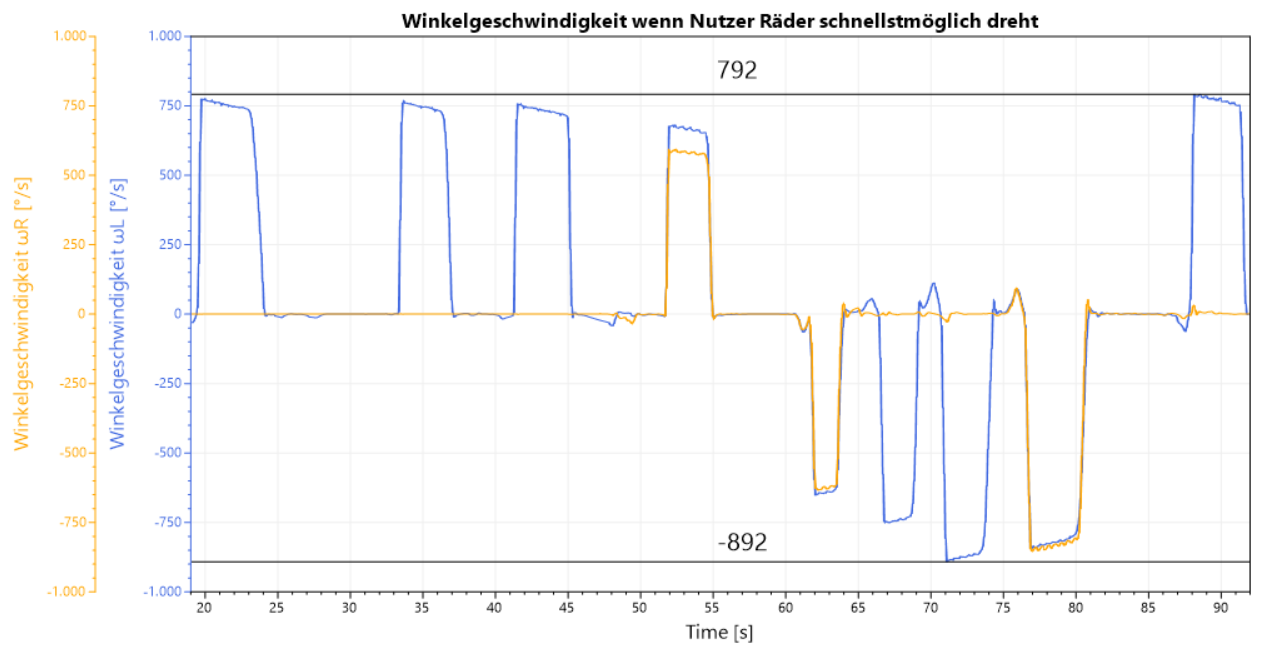
\includegraphics[width=\textwidth]{gyroMax.PNG}
    \caption{Bahngeschwindigkeiten im Verlauf der Zeit, bei dem die Testperson ein Rad, mit der dominanten Hand, so schnell wie möglich dreht}
\end{figure}

Das Diagramm zeigt bei einer Roation nach vorne einen maximal erreichten Ausschlag um $800\ \si{\degree}/s$.
Bei Rotationen nach hinten ist der Ausschlag etwas höher, übersteigt jedoch nicht $-900\ \si{\degree}/s$.
Daraus folgt, dass Gyroskop-Modus 2 für dieses Szenario der Ideale ist.
Bei diesem Modus ist die Maximale Gradzahl pro Sekunde $1000\ \si{\degree}/s$.
Der Nutzer erreicht nicht die maximal Geschwindigkeit und reizt trotzdem den Wertebereich ca. $80\ \%-90\ \%$ aus. Deshalb wird dieser Modus im System verwendet.

In vielen Anwendungen ist es von Vorteil oder angenehmer für den Nutzer, sich schnellstmöglich mit der maximalen Fortbewegungsgeschwindigkeit zu bewegen.
Auf Dauer ist es ermüdend, die Räder möglichst schnell drehen zu müssen.
Um den Nutzer zu entlasten, kann entweder der Fortbewegungsvektor $\vec{f}$ immer auf einen maximalen Thumbstick-Ausschlag abgebildet werden oder es wird ein weiterer Schwellenwert eingeführt, ab dem alle Eingaben als maximaler Thumbstick-Ausschlag abgebildet werden.

\section{ESP32}
Um den MPU-6050 betreiben und dessen Daten an eine Software übermitteln zu können, wird ein Mikrocontroller-Board benötigt.
Es muss die entsprechenden Register auslesen und mittels drahtloser Kommunikation versenden.
Auf dem Markt ist eine große Anzahl von Produkten für die verschiedensten Anwendungsgebiete erhältlich.
Im Rahmen dieser Arbeit wurde der Mikrocontroller ESP32 verwendet, das aktuelle Modell der Firma \textit{Espressif}.
Boards mit diesem Chip sind kostengünstig (ca. 8 Euro).
Zudem ist der ESP32 mit WiFi (802.11 b/g/n), Bluetooth (v4.2) und ESP-Now Unterstützung ausgestattet (S. 8-9)\cite{ESP32Datasheet2022}.
Verbaut wurde ein Xtensa® 32-bit LX6 Mikroprozessor, mit 240MHz Taktfrequenz, 448 KB ROM und 520 KB SRAM. (S. 32)\cite{ESP32Datasheet2022}
Als Entwicklungsboard wurde das ESP32 Dev Kit C V4 verwendet.

Der MPU-6050 muss wie folgt an das Entwicklungsboard angeschlossen werden:

\begin{table}[h]
    \centering
    \begin{threeparttable}
        \caption{Zuweisungs der jeweiligen Pins}
        \begin{tabular}{|l|l|}
            \hline
            \textbf{ESP32}                          & \textbf{MPU-6050}           \\ \hline
            \parbox[c][0.5cm]{3cm}{3.3V}            & \parbox[c][0.5cm]{3cm}{VCC} \\ \hline
            \parbox[c][0.5cm]{3cm}{GND}             & \parbox[c][0.5cm]{3cm}{GND} \\ \hline
            \parbox[c][0.5cm]{3cm}{GPIO22 (I2C CL)} & \parbox[c][0.5cm]{3cm}{SDA} \\ \hline
            \parbox[c][0.5cm]{3cm}{GPIO21 (I2C DA)} & \parbox[c][0.5cm]{3cm}{SCL} \\ \hline
            \parbox[c][0.5cm]{3cm}{ADO}             & \parbox[c][0.5cm]{3cm}{GND} \\ \hline
        \end{tabular}
    \end{threeparttable}
\end{table}

\section{3D gedruckte Box}
Damit Entwicklungsboard, Gyroskop und Akku zusammengehalten werden, geschützt sind und am Rad befestigt werden können, wird eine Box benötigt, die alle Komponenten aufnehmen kann und diese trägt.
Aufgrund dessen wurde – mithilfe von Blender – eine entsprechend seinen Anforderungen konstruierte Box entworfen und mittels 3D-Druckers gedrucht.

\section{Vergleich zwischen WiFi und ESP-Now}
Für die Übermittlung der Sensordaten an eine Software auf einem PC stehen, verschiedene Möglichkeiten zur Verfügung.
In dieser Arbeit sind zwei verschiedene Protokolle getestet worden: WiFi und ESP-Now. Die Protokolle müssen dabei leicht in das System integrierbar sein.
WiFi ist ein weit verbreiteter Standard, sodass entsprechende Bibliotheken schon existieren, um das Protokoll einbinden zu können\cite{WiFiArduinoReference}.
ESP-Now ist weniger verbreitet, da aber der Chip vom selben Hersteller kommt, existieren auch hier schon Bibliotheken, beziehungsweise ist die benötigte Bibliothek schon im Entwicklungspaket des Chips schon enthalten\cite{EspressifIoTDevelopment2022}.
Ein weiteres verfügbares Protokoll ist Bluetooth.
Jenes muss jedoch aufgrund des zeitlichen Rahmens dieser Arbeit, an anderer Stelle beleuchtet werden.

\subsection{WiFi und WebSockets}
WiFi ist eine Kommunikationstechnologie, die durch die WiFi-Alliance entstanden ist und bis heute von ihr gepflegt wird\cite{WhoWeAre}.
Sie ermöglicht drahtlose Kommunikation mit jedem Gerät, welches diese Technologie implementiert.
Inzwischen ist WiFi ein weit verbreiteter Standard, welcher von den meisten mobilen Geräten unterstützt wird\cite{DiscoverWiFiWiFi}.
Ein solches Gerät ist der ESP32.

Zunächst muss eine Verbindung zwischen dem ESP32 und dem lokalen Netzwerk mittels WiFi aufgebaut werden.
Damit die Zugangsdaten nicht fest in den Code geschrieben werden müssen, wird die Bibliothek \textit{WiFi Manager}\cite{tzapuWiFiManager2022} verwendet.
Diese baut selbstständig eine Verbindung mit einem Netzwerk auf, nachdem die Zugangsdaten über ein Gerät wie zum Beispiel einem Smartphone übergeben wurden.
Dazu wird ein Web-Konfigurations-Portal auf dem ESP32 gehostet, auf das ein nahes WiFi-fähiges Gerät zugreifen kann.

Für die eigentliche Übertragung der Daten können verschiedene Protokolle verwendet werden.
Ein klassischer Vertreter ist HTTP(S).
Dieses wurde für die vorliegende Arbeit jedoch nicht verwendet, da das Protokoll auf Hypertext ausgelegt ist.
Es wird für jede Abfrage von Daten eine neue TCP-Verbindung mit dem Server aufgebaut, der die Daten nach Eingang der Anfrage zurückschickt.
Will der Client neue Daten empfangen, so muss dieser erneut eine TCP-Verbindung mit dem Server aufbauen (S. 4)\cite{ietfRFC6455WebSocket}.
Zusätzlich enthält jedes Paket, welches vom Clienten kommt, viel Overhead, da jede dieser Nachrichten einen HTTP-Header besitzt (S. 4)\cite{ietfRFC6455WebSocket}.
Da es sich bei den Gyroskop-Daten jedoch um Echtzeitdaten handelt, wäre dieses Vorgehen ineffizient.
Viel Zeit und Bandbreite würde für das Übertragen von nicht benötigte Daten verwendet werden.

Eine Alternative ist die Verwendung von einem WebSocket.
Das Protokoll wurde entwickelt, um die Nachteile von HTTP(s) bei Echtzeitdaten zu umgehen und wird heute breit unterstützt.
Das WebSocket-Protokoll wurde in seiner finalen Form 2011 von der Internet Engineering Task Force entwickelt und veröffentlicht\cite{ietfRFC6455WebSocket}.
Dabei wird analog zu HTTP zu Beginn ein TCP Handshake durchgeführt. Der Client stellt an den Server eine Verbindungsanfrage, welcher dieser bestätigt.
Ab diesem Zeitpunkt sendet der Server unaufgefordert die vom Client abonnierten Daten, bis die Verbindung vom Client beendet wird (S. 5)\cite{ietfRFC6455WebSocket}.
Somit lassen sich höhere Datenraten erzielen, die für Echtzeitanwendungen notwendig sind.
Das für die vorliegende Bachelor-Thesis entwickelte System setzt auf einen vom ESP32 gehosteten WebSocket-Server, der von der Software auf dem PC abonniert wird.
Dabei kommt aufseiten des ESP die Bibliothek \textit{arduinoWebSockets}\cite{markusWebSocketServerClient2022} zum Einsatz, und auf der Client Seite die Bibliothek \textit{websocket-client}\cite{kotasWebsocketclient2022}.

Zusätzlich zur eigentlichen Übertragung der Daten ist es notwendig, dass die Software auf dem PC den IP-Endpunkt des WebSockets auf dem ESP32 kennt.
Dazu sendet der Mikrocontroller ebenfalls über WiFi einen UDP-Broadcast ins Netzwerk.
Neben dem IP-Endpunkt werden auch Informationen über das Gerät mitgesendet, damit die Software auf dem PC weiß, um welches Gerät es sich handelt.
Nach dieser Bekanntmachung kann der WebSocket abonniert und die Daten übertragen werden.

\subsection{ESP-Now und Serieller Port}
ESP-Now ist ein vom Unternehmen \textit{Espressif} selbst entwickeltes Übertragungsprotokoll, mit dem Mikrocontroller von \textit{Espressif} wie zum Beispiel der ESP8266 (Vorgänger des ESP32) und der ESP32 direkt miteinander Daten austauschen können.
Dabei verwendet das Protokoll die MAC-Adressen zur Identifikation der Geräte.
Es wird jedoch nur eine Verbindung in eine Richtung aufgebaut.
Ein großer Vorteil dieses Protokolls ist die unkomplizierte Einbindung in das System.
Anders als WiFi muss nicht zunächst eine Verbindung zu einem Netzwerk aufgebaut werden, sondern dem Gerät muss lediglich die MAC-Adresse des Zielgeräts vorliegen.
Da die Kommunikation jedoch nur unter Mikrocontrollern stattfindet, muss das Gerät, welches die Sensor-Daten entgegennimmt, diese Daten mittels seriellen Ports an die Software auf dem PC übertragen.
Damit steigt die Anzahl der Verbindungen, an denen die Übertragung scheitern kann.
Jedoch erleichtert es die Verwendung für den Endbenutzer, da dieser kein WiFi-Netzwerk benötigt, um die Geräte mit der Software auf dem PC zu verbinden.
Eine Verbindung per USB-Kabel ist ausreichend.

\section{Analyse der Messungen}
Damit der Nutzer eine präzise Eingabe tätigen kann, ist es notwendig, dass möglichst schnell und kontinuierlich neue Pakete empfangen werden.
Um die Datenrate zu ermitteln, mit der beide Nodes (eingebettete Systeme an den Rädern) die Gyroskop-Werte verschicken, wird clientseitig alle 250ms die aktuelle Datenrate errechnet.
Dazu zählt die Software seit der letzten Messung die eingegangenen Pakete und multipliziert diese mit 4, um die Datenrate pro Sekunde zu erhalten.
Zusätzlich wird bei jedem Datensatz ermittelt, wie viel Zeit zwischen den letzten beiden Paketen vergangen ist.
Auf die Messung der Latenz wird im Hinblick auf den Umfang der Arbeit verzichtet, da dies erfodert hätte beide Seiten der Verbindung zu synchronisieren.

\begin{figure}[h]
    \centering
    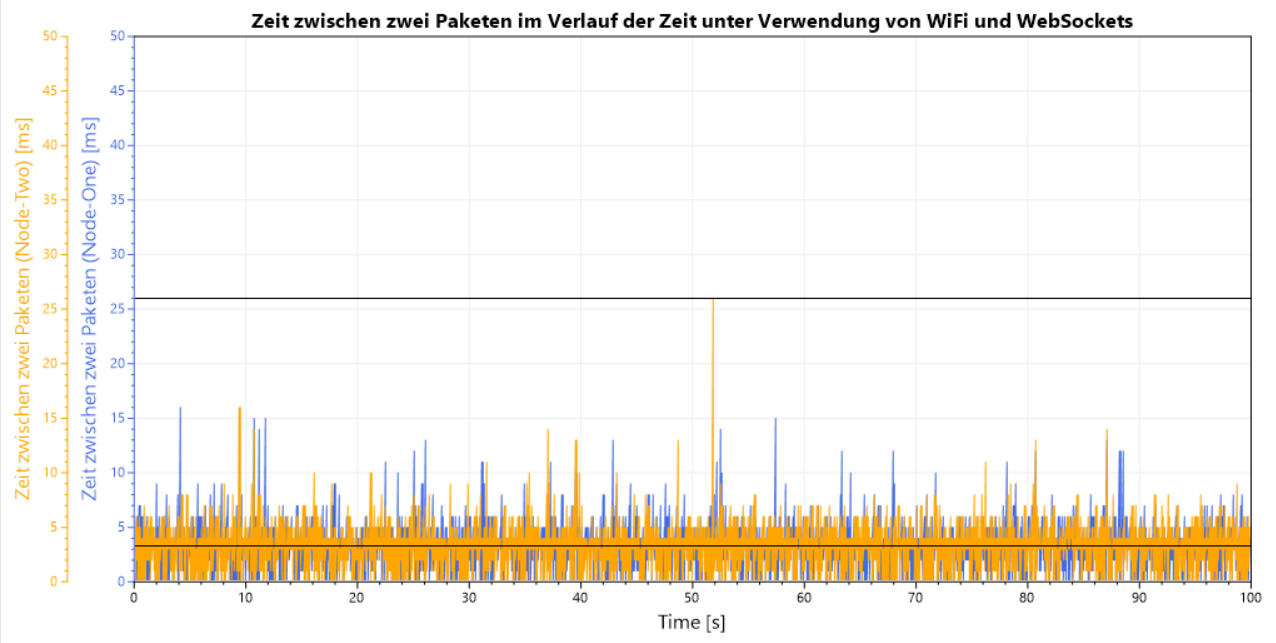
\includegraphics[width=\textwidth]{wifiStats.PNG}
    \caption{Intervall zwischen Paketen im Verlauf der Zeit bei WiFi}
    \label{fig:wifiStats}
\end{figure}
\begin{figure}[h]
    \centering
    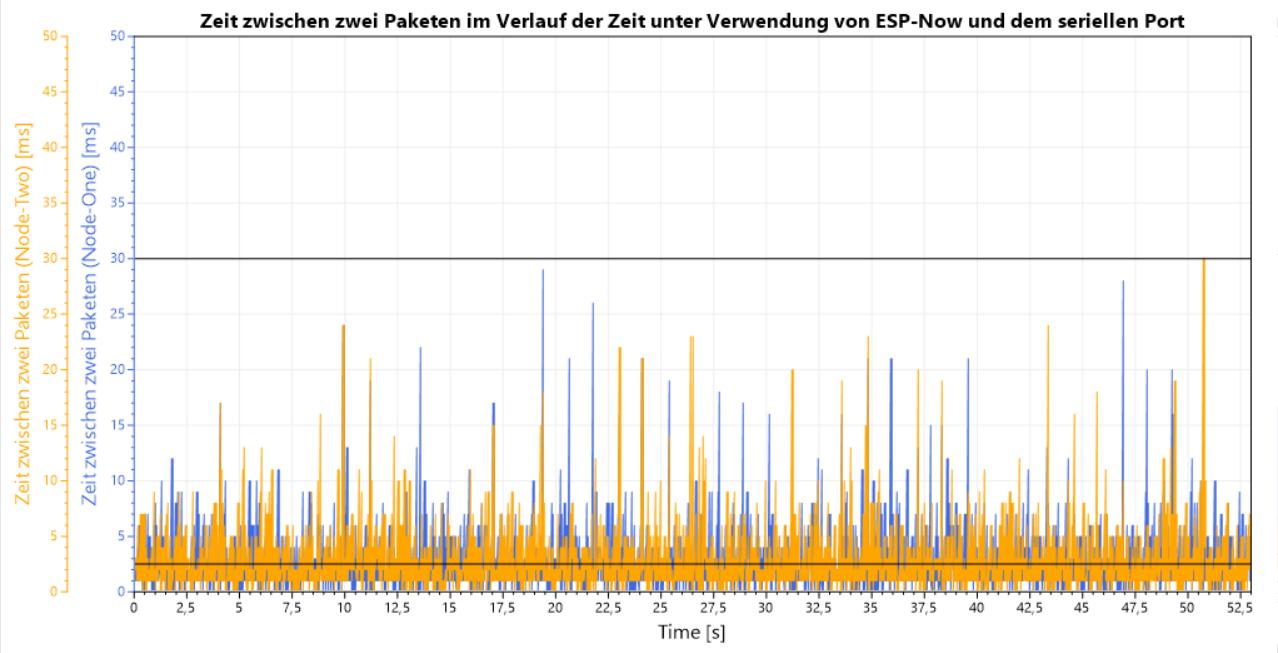
\includegraphics[width=\textwidth]{espnowStats.PNG}
    \caption{Intervall zwischen Paketen im Verlauf der Zeit bei ESP-Now}
    \label{fig:espnowStats}
\end{figure}

\begin{table}[h]
    \centering
    \begin{threeparttable}
        \caption{Messungen der getesteten Verbindungsmethoden}
        \begin{tabular}{|l|l|l|}
            \hline
            ~                                                                 & \parbox[c][1.5cm]{2cm}{\textbf{WiFi          \\mit\\WebSocket}} & \parbox[c][1.5cm]{2.5cm}{\textbf{ESP-Now\\mit\\seriellem Port}} \\ \hline
            \parbox[c][0.5cm]{6cm}{\textbf{Pakete pro Sekunde Durchschnitt} } & 250,16                              & 330,43 \\ \hline
            \parbox[c][0.5cm]{6cm}{\textbf{Pakete pro Sekunde Minimum}      } & 220                                 & 204    \\ \hline
            \parbox[c][0.5cm]{6cm}{\textbf{Pakete pro Sekunde Maximum}      } & 284                                 & 440    \\ \hline
            \parbox[c][0.5cm]{6cm}{\textbf{Paketintervall Durchschnitt [ms]}} & 3,09                                & 2,52   \\ \hline
            \parbox[c][0.5cm]{6cm}{\textbf{Paketintervall Minimum [ms]}     } & <1                                  & <1     \\ \hline
            \parbox[c][0.5cm]{6cm}{\textbf{Paketintervall Maximum [ms]}     } & 26                                  & 30     \\ \hline
        \end{tabular}
    \end{threeparttable}
\end{table}

Die Messungen haben ergeben, dass die Zeit zwischen zwei Paketen im Schnitt im niedrigen einstelligen Millisekundenbereich sind.
ESP-Now mit seriellem Port schafft dabei im Durchschnitt 80 Pakete mehr als WiFi mit einem WebSocket.
Die Verbindung mit WiFi ist jedoch deutlich störungsfreier.
So ist aus Abbildung \ref{fig:espnowStats} abzulesen, dass entweder ESP-Now oder der serielle Port regelmäßiger und höhere Ausreißer erzeugt, bei denen die Zeit zwischen zwei Paketen über 15 Millisekunden ist.
WiFi hingegen hat im kompletten Datensatz nur einen deutlichen Ausreißer und hat ansonsten selten Zeiten über 15 Millisekunden. Es kann geschlussfolgert werden, dass WiFi vorzuziehen ist.
Jedoch kann auf ESP-Now mit seriellem Port zurückgegriffen werden, wenn nur ein USB-Anschluss und kein WiFi Netzwerk verfügbar ist.
Anzumerken ist jedoch, dass die Messungen stark abhängig davon sind, welche USB-Anschlüsse und -Protokolle verwendet wurden, sowie welche Datenraten der Router unterstützt.
Ein weiterer Einflussfaktor ist die Verbindung zwischen Client und dem Router.
Sind diese kabellos verbunden, erhöht sich zusätzlich die Zeit, die ein Paket zur Übertragung benötigt, im Gegensatz zur kabelgebundener Übertragung.
Deshalb sind die erhobenen Messwerte nur begrenzt aussagekräftig.
Trotzdem lässt sich erkennen, dass beide Methoden genug Pakete verschicken können, um eine flüssige Bewegung nativ aus den Daten berechnen zu können.
Es sind keine Interpolationstechniken notwendig, um die Bewegung flüssig erscheinen zu lassen.

\newpage

\begin{table}[t]
    \centering
    \begin{threeparttable}
        \caption{Die Verbindungsmethoden im Vergleich}
        \begin{tabular}{|m{2.8cm}|m{3cm}|m{4cm}|}
            \hline
            ~                                                     & \parbox[c][1cm]{3cm}{\textbf{WiFi \\mit WebSocket}} & \parbox[c][1cm]{4cm}{\textbf{ESP-Now\\mit seriellem Port}} \\ \hline
            \parbox[c][1cm]{2.8cm}{\textbf{Anzahl                                                     \\Mikrocontroller}} & 2                                                     & 3 \\ \hline
            \parbox[c][3cm]{2.8cm}{\textbf{Daten-Pfad}}           & \parbox[c]{3cm}{\shortstack{ESP32 \\$\downarrow$     \\Router\\$\downarrow$ \\Rollstuhl-Software}}                            & \parbox[c]{3cm}{\shortstack{ESP32\\$\downarrow$\\ ESP32\\$\downarrow$\\ Serieller-Port\\$\downarrow$\\ Rollstuhl-Software}}   \\ \hline
            \parbox[c][2cm]{2.8cm}{\textbf{"Hardcoding"                                               \\von\\Verbindungs-\\Informationen}} & nicht notwendig & Ziel-MAC-Adressen \\ \hline
            \parbox[c][3.5cm]{2.8cm}{\textbf{Vorteile}}
                                                                  &
            \parbox[c][3cm]{4cm}{
            \begin{itemize}
                    \item Stabilere\\Verbindung
                    \item Nur eine\\Übertragungs\\-technologie\\notwendig
                \end{itemize}} &
            \parbox[c][3.5cm]{4cm}{
            \begin{itemize}
                    \item Kein Verbindungsaufbau mit lokalem Netzwerk notwendig
                    \item Kein WiFi-Netzwerk notwendig, ein USB-Anschluss genügt
                \end{itemize}}                               \\ \hline
        \end{tabular}
    \end{threeparttable}
\end{table}
\chapter{Abbildung der empfangenen Daten auf ein Eingabegerät}
Nachdem die Daten des eingebetteten Systems zur Rollstuhl-Software übermittelt wurden, müssen diese nun auf auf ein herkömmliches Eingabegerät abgebildet werden.
Es wird sich der Frage gewidmet, welches Eingabegerät in Frage kommt und wie möglichst viele, präzise Eingaben auf dieses Eingabegerät abgebildet werden können.
Im letzten Teil des Kapitels werden aufgenommene Datenreihen untersucht, um fehlerhafte Eingaben zu minimieren.

\section{Interface zur Nutzung der Rad-Daten in externer Software}
Die Raddaten, welche die Rollstuhl-Software empfangen hat, müssen nun zu externer Software gelangen.
Dazu ist eine vorhandene Schnittstelle notwendig (Tastatur, Maus, Spielcontroller, ...), denn es kann nicht davon ausgegangen werden, dass jede externe Software eine neue Schnittstelle implementiert.
Jedoch muss in diesem Fall, in der Rollstuhl-Software eine Abbildung auf eine vorhandene Schnittstelle durchgeführt werden.

\subsection{Vergleich zwischen Tastatur und Spielcontroller}
Tastaturen und Spielcontroller werden von den meisten Anwendungen unterstützt und eignen sich unterschiedlich gut für die Zwecke des hier entwickelten Systems.
Tastatureingaben bieten den Vorteil, dass sie von fast jeder erdenklichen Software unterstützt werden. Jedoch lassen nur binäre Eingaben, durch das Drücken von Tasten tätigen.
Da die Rollstuhl-Eingaben jedoch unterschiedliche Werte innerhalb eines Wertebereichs darstellen, wird bei einer Tastatureingabe die Interaktionsmöglichkeit stark eingeschränkt.
Zudem ist oft das zusätzliche Verwenden einer Maus erforderlich. Dies verkompliziert das Abbilden zusätzlich.
Die Alternative ist ein Mapping auf eine Spielcontroller-Eingabe.
Hier gibt es ebenfalls Knöpfe, beziehungsweise binäre Eingaben, aber auch Eingaben entlang von Achsen innerhalb eines Wertebereichs.
Überwiegend werden die Achsen in Form eines Thumb-Sticks oder Knopfes mit mehreren Stufen realisiert.
Auf der einen Seite könnten so Rollstuhl-Eingaben, wie das Fortbewegen, einfacher auf das Gerät abgebildet werden.
Andererseites unterstützt nicht jede Software Eingaben mittels eines Spielcontrollers.
Es wurde sich im Rahmen dieser Arbeit für das Abbilden auf, und emulieren von, einem Spielcontroller entschieden.
Grund dafür ist, dass die meiste Software in der Fortbewegung eine Rolle spielt (meist Computerspiele oder andere 3D-Räume), diese unterstützen.

\subsection{Emulation des Spielcontrollers}
Um die Eingaben des Rollstuhls in tatsächliche Spielcontroller-Eingaben umzuwandeln, die vom Betriebssystem auch als Controller-Eingabe verstanden werden, ist eine Emulation eines Controllers notwendig.
Ziel ist es, programmgesteuert Controller-Eingaben an den Rechner zu senden.
Um sich den Aufwand des Schreibens eines neuen Treibers zu ersparen, wird an dieser Stelle auf das \textit{Virtual Gamepad Emulation Framework}\cite{VirtualGamepadEmulation} zurückgegriffen.
Dies ist eine Bibliothek, welche in bestehende Software integriert werden kann und einen virtuellen Controller mit dem Rechner verbindet.
Über Befehle lassen sich anschließend Controller-Eingaben tätigen.
Das Framework unterstützt Xbox 360-, sowie DualShock 4-Controller\cite{VirtualGamepadEmulationa}.

Die Internet-Vertriebsplattform Steam, welche hauptsächlich Computerspiele vertreibt, hat eine Umfrage veröffentlicht, über die Verteilung von Spielcontrollern auf ihrer Platform.
Der Abbildung \ref{tab:connectionStats} ist zu entnehmen, dass $45\ \%$ aller Controller ein Xbox 360 Controller sind\cite{SteamSteamNews2018}.
%Zusätzliche $19\ \%$ aller Controller sind ein Xbox One Controller, ein Modell welches seinem Vorgänger sehr ähnlich ist.
Damit sind sie mit großem Abstand am verbreitetsten.
Aufgrund dessen wurde sich im Rahmen der vorliegenden Arbeit für die Emulation eines Xbox 360 Controllers entschieden, da anzunehmen ist, dass dieser Controller am wahrscheinlichsten unterstützt wird.

\begin{figure}[h]
    \centering
    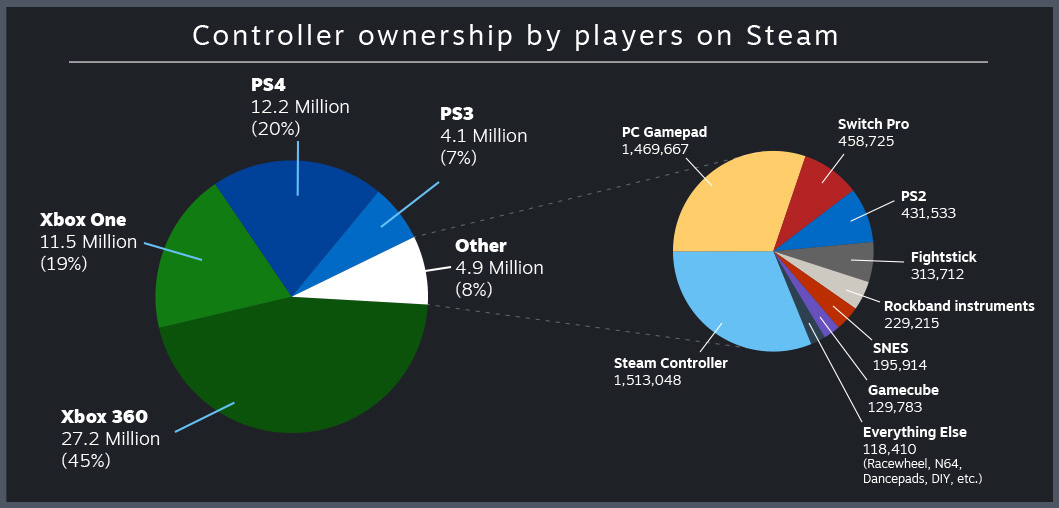
\includegraphics[width=\textwidth]{steamControllerStatistik.jpg}
    \caption{Verteilung von Besitz von verschiedenen Spielcontrollern auf der Plattform Steam\cite{SteamSteamNews2018}}
    \label{fig:controllerStats}
\end{figure}

\section{Algorithmen zur Abbildung der Rad-Daten in Controller-Eingaben}
Die Sensor-Daten der Gyroskope liefern die Winkelgeschwindigkeiten der Räder des Rollstuhls.
Diese sollen – wie bereits in Kapitel 5.3.1 beschrieben – auf die Eingabemöglichkeiten eines Spielcontrollers abgebildet werden, um sich im virtuellen Raum bewegen oder andere Eingaben tätigen zu können.
Die Abbildung erfolgt dabei auf einen Xbox360 Controller. Somit sind die abgebildeten Eingaben von jeder Software lesbar, die eine Xbox360 Controllerunterstützung implementiert haben.
Die in diesem Kapitel werden gelgentlich Aussagen getroffen die mit dem Emfinden des Nutzers zu tun haben oder von ihm abhängig sind.
Da subjektive Eindrücke nur schwer und unpräzise gemessen werden können, leidet dadurch an manchen Stellen die Aussagekraft.
Darüber hinaus konnten nur wenige Personen im Umkreis des Erstellers dieser Arbeit als Testperson verwendet werden, was zusätzlich einzelne Aussagen abschwächt.
Eine zukünftige Arbeit muss sich ausführlicher an diesen Stellen mit den Betreffenden Fragen befassen, und einen größeren diverseren Pool aus Testpersonen verwenden, um die Aussagekraft zu erhöhen.

\subsection{Abbildung auf einen Thumbstick}
Der direkte Weg die Raddaten in eine Eingabe umzuwandeln ist, diese auf jeweils eine Achse eines Thumbsticks abzubilden.
Anwendungsgebiet von dieser Art von Abbildung ist, die Steuerung eines Cursors.
Dabei wird die x-Achse mit dem einen, die y-Achse mit dem anderen Rad dargestellt.
Vorteilig ist dabei, dass beide Achsen gleichzeitig angesprochen werden können.
Jedoch ist es schwieriger, die x-Achse zu bewegen, da sie anders ausgerichtet ist als das Rad, das gedreht wird.
Alternativ kann das Ansprechen einer Achse auch durch beide Räder passieren.
Dabei wird die x-Achse dann angesprochen, wenn sich die Räder gegeneinander drehen und die y-Achse, wenn sich die Räder miteinander drehen.
Damit wird eine intuitive Nutzung angestrebt.
Jedoch ist es dabei nicht mehr möglich, gleichzeitig den Cursor entlang beider Achsen zu bewegen, da sich die Räder nicht gleichzeitig mit- und gegeneinander drehen können.

\subsection{Abbildung auf einen simulierten Rollstuhl}
Da das im Rahmen dieser Arbeit entwickelte System darauf abzielt, in einem dreidimensionalen virtuellen Raum, auf einer Ebene zu navigieren, wird eine Abbildung benötigt, die die Position des Nutzers im virtuellen Raum verändert.
Da die Daten ohnehin von einem Rollstuhl kommen, liegt die Abbildung auf einen simulierten Rollstuhl nahe.
Um die Raddaten der zwei Räder auf eine Bewegung und Rotation eines Rollstuhls umzurechnen, muss erst festgestellt werden, welche Drehbewegungen zu welchen Rollstuhlbewegungen führt.
Dabei können vier vereinfachte Fälle unterschieden werden:

\begin{figure}[h]
    \centering
    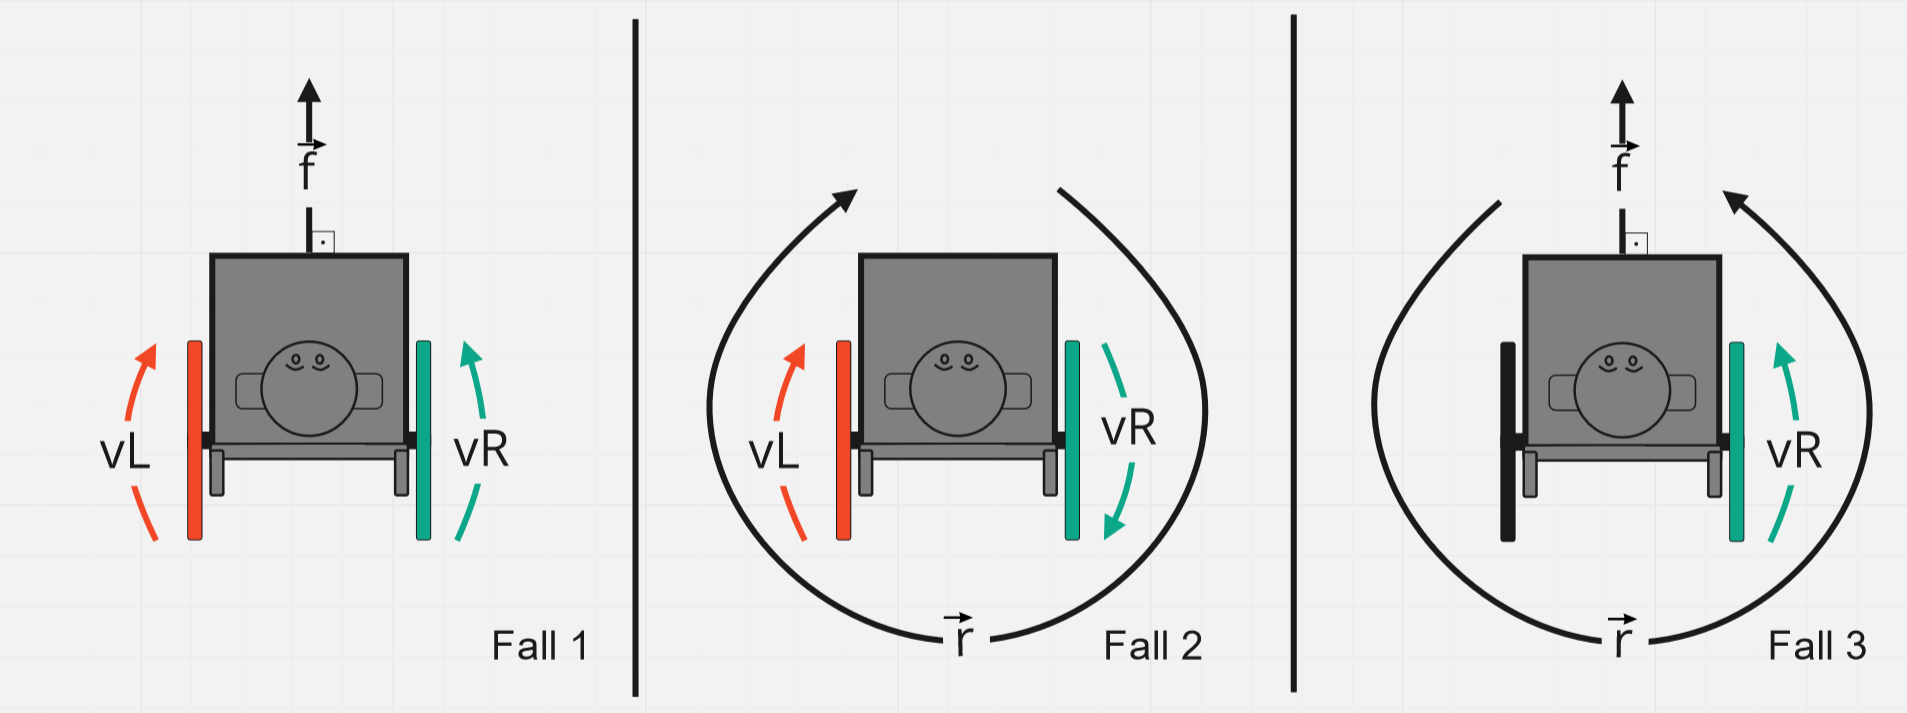
\includegraphics[width=\textwidth]{wheelchairCases.PNG}
    \caption{Die Bewegungs-Fälle des Rollstuhl aus der Vogelperspektive}
    \label{fig:wheelchairCases}
\end{figure}

\textbf{Fall 1:} Drehen sich die Räder mit gleicher Geschwindigkeit in dieselbe Richtung, so ruft dies eine Bewegung nach vorne oder hinten aus (Abbildung \ref{fig:wheelchairCases}, Fall 1).

\textbf{Fall 2:} Drehen sich die Räder mit gleicher Geschwindigkeit gegeneinander, so ruft dies eine Rotation um die eigene Achse hervor (Abbildung \ref{fig:wheelchairCases}, Fall 2).

\textbf{Fall 3:} Dreht sich nur ein Rad, so dreht sich dieses um das Stehende (Abbildung \ref{fig:wheelchairCases}, Fall 3).

\textbf{Fall 4:} Drehen sich die Räder unterschiedlich schnell, so muss die Bewegung zusammengesetzt werden aus den Bewegungskomponenten einer der ersten beiden Fälle und dem dritten Fall.

Im Folgenden wird die Berechnung der Bewegungsanteile aufgezeigt, bestehend aus Bewegung nach vorne/hinten und der Rotation um die eigene Achse:

\begin{align}
    \omega_L      & : \ \mathrm{Winkelgeschwindigkeit\ des\ linken\ Rades}\ [\si{\degree/\second}]  \\
    \omega_R      & : \ \mathrm{Winkelgeschwindigkeit\ des\ rechten\ Rades}\ [\si{\degree/\second}] \\
    m             & : \ \mathrm{Winkelgeschwindigkeit\ Minimum}\ [\si{\degree/\second}]             \\
    o             & : \ \mathrm{Overshoot}\ [\si{\degree/\second}]                                  \\
    d             & : \ \mathrm{Abstand\ Der\ R\ddot{a}der}\ [\si{\metre}]                          \\
    \vec{f}       & : \ \mathrm{Fortbewegungsvektor}\ [\si{\metre/\second}]                         \\
    \vec{r}       & : \ \mathrm{Rotationsvektor}\ [\si{\metre/\second}]                             \\
    \vec{f_{1,2}} & : \ \mathrm{Fortbewegungsvektor\ Fall1\ oder\ Fall2}\ [\si{\metre/\second}]     \\
    \vec{r_{1,2}} & : \ \mathrm{Rotationsvektor\ Fall1\ oder\ Fall2}\ [\si{\metre/\second}]         \\
    \vec{f_{3}}   & : \ \mathrm{Fortbewegungsvektor\ Fall3}\ [\si{\metre/\second}]                  \\
    \vec{r_{3}}   & : \ \mathrm{Rotationsvektor\ Fall3}\ [\si{\metre/\second}]
\end{align}

\begin{figure}[h]
    \centering
    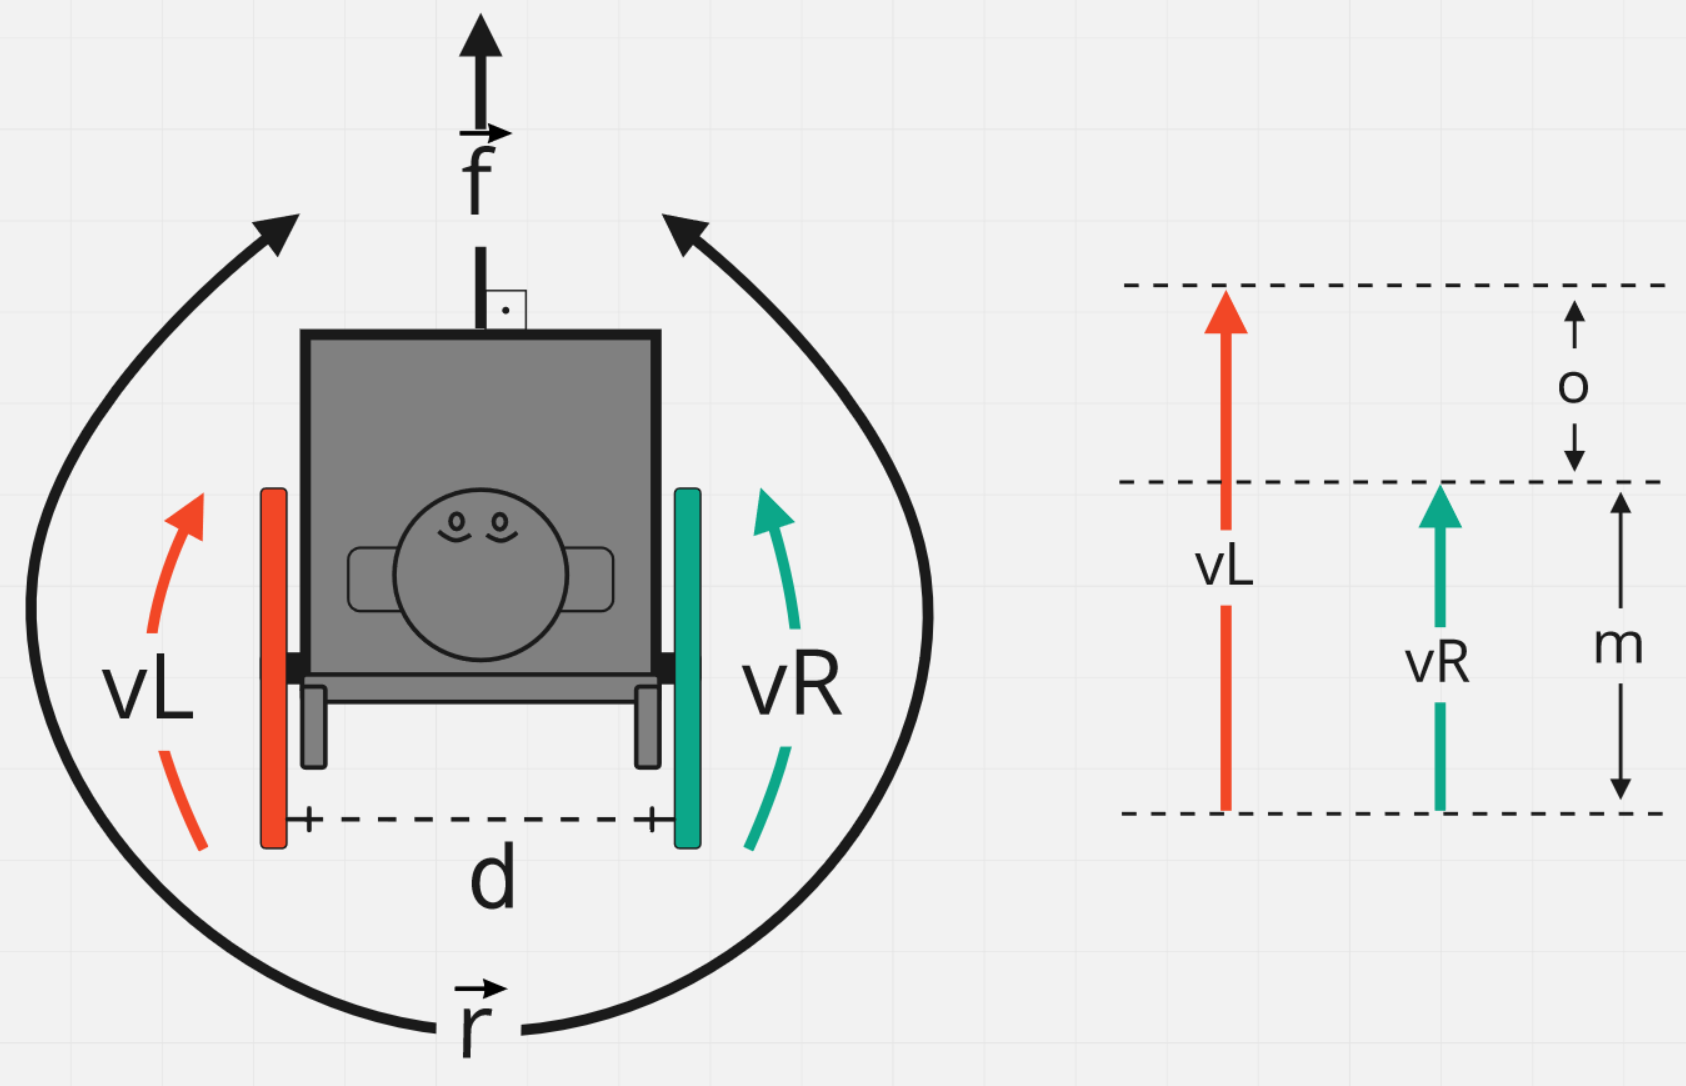
\includegraphics[width=0.75\textwidth]{WheelchairMath.PNG}
    \caption{Skizze des Rollstuhls aus der Vogelperspektive mit Bewegungsvektoren}
    \label{fig:wheelchairMath}
\end{figure}

Zunächst müssen die Rotationen der Räder dekonstruiert werden.
Dabei lässt sich die Rotation eines Rades in zwei Komponenten aufspalten (siehe Abbildung \ref{fig:wheelchairMath}).
Zum einen in den Minimum-Anteil $m$, den sich beide Räder drehen,
\begin{align}
    m = \min{(\left| \omega_L \right|,\left| \omega_R\right|)}
\end{align}

zum anderen in den Overshoot-Anteil $o$, den sich ein Rad schneller dreht als das andere.
\begin{align}
    o = \left|\left| \omega_L \right|-\left| \omega_R\right| \right|
\end{align}

\textbf{Fall 1:}
Die Bewegung nach vorne oder hinten (Fortbewegungsvektor Fall1 oder Fall2 $f_{1,2}$) ergibt sich in diesem Fall aus dem Anteil der Geschwindigkeit, mit denen sich beide Räder drehen.
Dabei dreht sich jedoch der Rollstuhl nicht.
\begin{align}
    \vec{f_{1,2}} = & \ m \\
    \vec{r_{1,2}} = & \ 0
\end{align}

\begin{figure}[h]
    \centering
    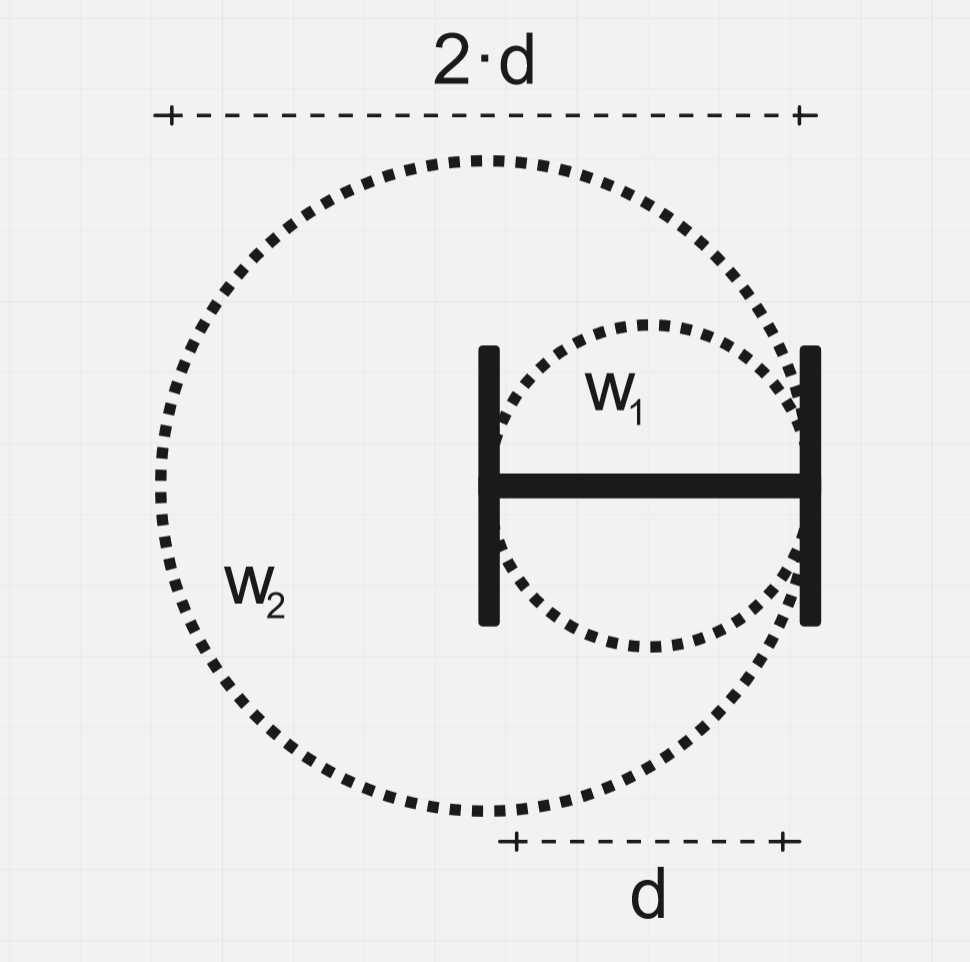
\includegraphics[width=0.5\textwidth]{wendekreis.PNG}
    \caption{Skizze des Rollstuhls aus der Vogelperspektive mit Wendekreisen}
    \label{fig:wendekreis}
\end{figure}

\textbf{Fall 2:}
Zur Berechnung der Rotation um die eigene Achse wird zunächst der Wendekreis $w_1$ benötigt.
Dieser Wendekreis ist abhängig vom Abstand der Räder $d$ und dessen Mittelpunkt liegt im Mittelpunkt zwischen den Rädern (siehe Abbildung \ref{fig:wendekreis}).
Anschließend wird mithilfe des Minimums $m$, das Verhältnis von $m$ zu $w_1$ errechnet, also wie viel vom Wendekreis gedreht wird.
Dieses Verhältnis muss zum Schluss mit $360$ multipliziert werden, um den resultierenden Winkel, beziehungsweise Rotationsvektor Fall1 oder Fall2 $r_{1,2}$, zu berechnen.
Bei dieser Bewegung verändert der Rollstuhl jedoch nicht seine Position.
\begin{align}
    w_1           & =            \ d \cdot \pi                  \\
    \vec{r_{1,2}} & =  \ \left(\frac {m} {w_1}\right) \cdot 360 \\
    \vec{f_{1,2}} & =  \ 0
\end{align}

\textbf{Fall 3:}
Bei diesem Fall gibt es einen Fortbewegungs- und einen Rotationsvektor ungleich null.
Da sich nur ein Rad bewegt, hat sich der Wendekreis vergrößert zu $w_2$.
Der Durchmesser von $w_2$ ist nun doppelt so groß wie von $w_1$, da das stehende Rad nun der Mittelpunkt des Wendekreises ist.
Jetzt wird der Overshoot $o$ (also der Anteil der Bewegung des Rades, das sich mehr als das andere dreht) ins Verhältnis gesetzt mit $w_2$ und erhält dadurch $\Theta$.
Verrechnet man $\Theta$ mit dem inneren Wendekreis $w_1$, so erhält man den Fortbewegungsvektor Fall3 $f_3$.
\begin{align}
    w_2 =       & \ 2 \cdot d \cdot \pi \\
    \Theta =    & \ \frac {o} {w_2}     \\
    \vec{f_3} = & \ \Theta \cdot w_1
\end{align}

Um den Rotationsvektor Fall3 $r_3$ berechnen zu können, muss $\Theta$ mit $360$ multipliziert werden.
\begin{align}
    \vec{r_3} = \Theta \cdot 360
\end{align}

Da die Berechnungen mit den absoluten Rotationswerten errechnet wurden, ist es notwendig anhand der Drehrichtungen beider Räder zu bestimmen, ob sich der Rollstuhl vor- oder zurückbewegt und ob er sich dabei nach links oder rechts dreht.
Die Drehrichtung ist immer dann links, wenn:
\begin{align}
    \omega_L < \omega_R
\end{align}

sonst ist sie rechts.
Es handelt sich um eine Vorwärtsbewegung, wenn:
\begin{align}
    \omega_L + \omega_R > 0
\end{align}

sonst ist es eine Rückwärtsbewegung.
Folgende Bedingungen können vernachlässigt werden, da sie in der Realität nur Auftreten wenn der Overshoot $o = 0$ ist und damit $\vec{f_3} = 0$ und $\vec{r_3} = 0$:
\begin{align}
    \omega_L =            & \ \omega_R \\
    \omega_L + \omega_R = & \ 0
\end{align}

\textbf{Fall 4:}
Bevor die zusammengehörenden Vektoren zusammengerechnet werden können, muss überprüft werden, ob $s_{1,2}$ und $r_{1,2}$ mithilfe des ersten oder zweiten Falls berechnet werden müssen.
Gilt folgende Bedingung, drehen sich die Räder gegeneinander und es wird Fall 2 benötigt.
Andernfalls gilt Fall 1.
\begin{align}
    (\omega_L > 0) \oplus (\omega_R > 0)
\end{align}

Anschließend können die Bewegungskomponenten addiert werden:
\begin{align}
    \vec{s} = & \ \vec{f_{1,2}} + \vec{f_3} \\
    \vec{r} = & \ \vec{r_{1,2}} + \vec{r_3}
\end{align}

Sind die Bewegungskomponenten berechnet muss final eine Abbildung dieser auf den Spielcontroller erfolgen.
Dabei bietet sich die y-Achse des linken-Thumbsticks an für den Fortbewegungsvektor $\vec{s}$ und die s-Achse des rechten Thumbsticks für den Rotationsvektor $\vec{r}$.
In vielen Anwendungen, im besonderen 3D-Videospielen, ist der linke Thumbstick für das Bewegen im Raum zuständig und der rechte für das Umschauen.

Berechnet man auf Grundlage der oben genannten Formeln die Bewegung des Rollstuhls, so stößt man auf folgendes Problem:
Da die Räder bei einer beabsichtigten Bewegung nach vorne meist mit leicht unterschiedlicher Geschwindkeit drehen, erfährt der simulierte Rollstuhl eine Ablenkung nach rechts oder links.
Eine Ausrichtung des Rollstuhls, die der Nutzer gezielt vorgenommen hat, um ein bestimmtes Ziel im virtuellen Raum zu erreichen, ist damit nichtig, da der Rollstuhl sein Ziel verfehlt.
Bildet man den Durchschnitt $v$ der Rotationen beider Räder und nutzt ihn anstelle vom $Minimum\ m$, so verhindert man die unbeabsichtigte Ablenkung.
\begin{align}
    \vec{v} = \frac {(\omega_L + \omega_R)} {2}
\end{align}

Verwendet man den Durchschnitt $v$ müssen die verschiedenen Fälle distinkt sein, da sonst das Wenden mit einem Rad nicht mehr möglich wäre.
Grund dafür ist der zusammenaddierter Mittelwert der Geschwindigkeiten des stillstehenden und des sich drehenden Rades.
Dieser würde anstelle einer Drehung zu einer Vorwärtsbegung führen.
Das Zusammenrechnen von Fall 1 oder Fall 2, mit Fall 3 darf also nicht geschehen.
Um dies zu realisieren, sind Bewegungszustände notwendig.
Auf Basis dieser kann entschieden werden, welcher Fall genutzt werden muss, um die resultierende Bewegung zu errechnen.
Im nächsten Kapitel wird darauf eingegangen, welche Bewegungszustände existieren und wie diese erkannt werden können.

\subsection{Bewegungszustände}
Um alle Bewegungszustand-Permutationen ermitteln zu können, muss festegestellt werden, dass sich ein Rad in drei Zuständen befinden kann: Still stehend, nach vorne drehend und nach hinten drehend.
Zwei Räder mit jeweils drei Zuständen ergeben dabei neun Bewegungszustände ($3^2 = 9$), welche in Abbildung \ref{fig:wheelstates} skizziert sind.

\begin{figure}[h]
    \centering
    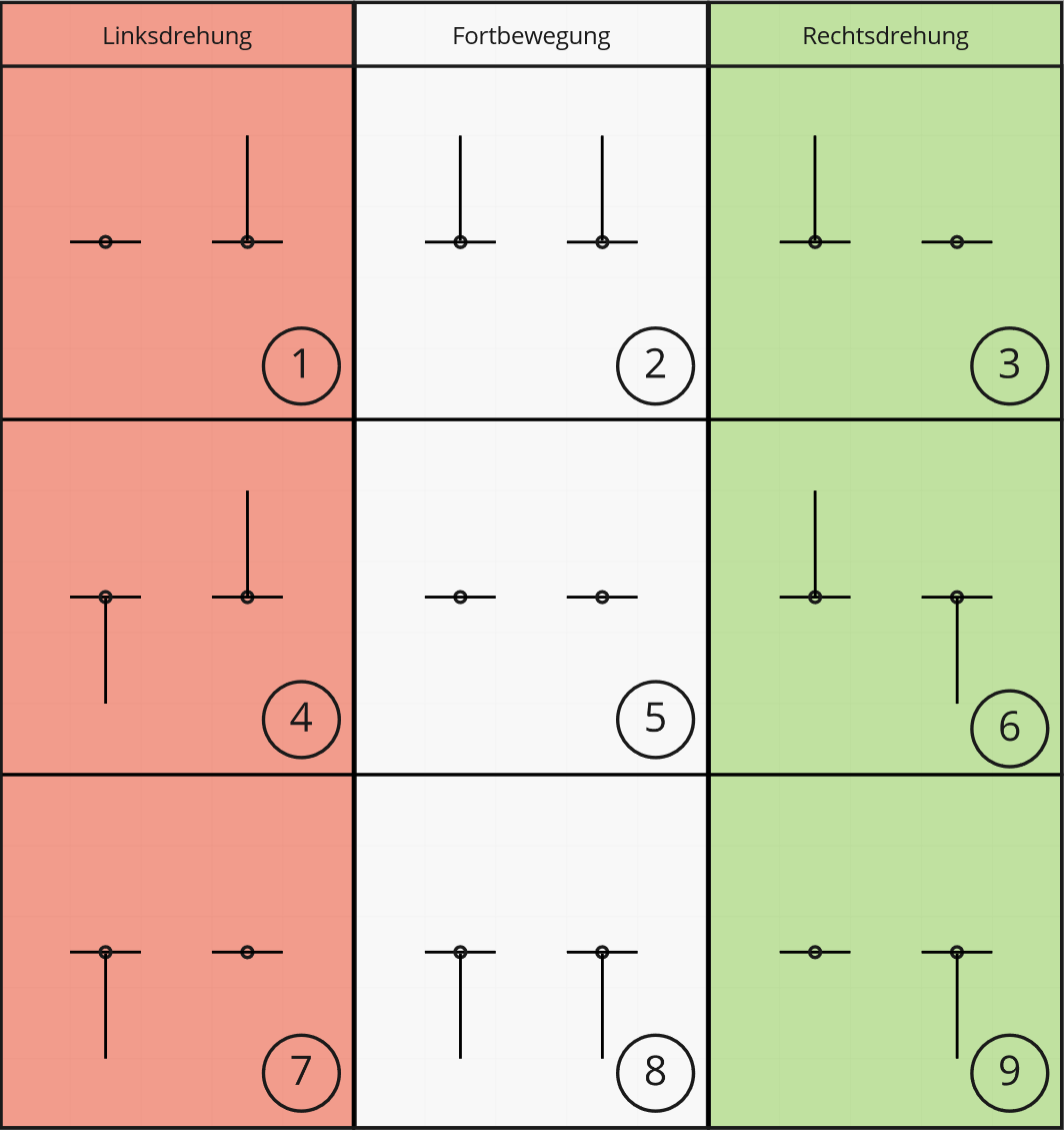
\includegraphics[width=0.75\textwidth]{WheelchairStates.PNG}
    \caption{Die neun Bewegungszustände eines Rollstuhls}
    \label{fig:wheelstates}
\end{figure}

Jedoch lässt sich die Menge von Bewegungszuständen in folgende disjunkte Teilmengen unterteilen:
\begin{itemize}
    \item \textit{Ruhezustand}: kein Rad dreht sich (5)
    \item \textit{Rotation um die eigene Achse}: Räder drehen sich gegeneinander (4, 6)
    \item \textit{Einzelradbewegung}: ein Rad steht still und ein Rad dreht sich (1, 3, 7, 9)
    \item \textit{Sichtachsenbewegung}: Räder drehen sich in dieselbe Richtung (2, 8)
\end{itemize}

Im Folgenden wird darauf eingegangen, wie diese Teilmengen-Zustände erkannt werden:
\begin{align}
    \omega_L & :\ \mathrm{Winkelgeschwindigkeit\ des\ linken\ Rades}  \\
    \omega_R & :\ \mathrm{Winkelgeschwindigkeit\ des\ rechten\ Rades} \\
    s        & :\ \mathrm{Schwellenwert}
\end{align}

\textbf{\textit{Ruhezustand}}\\
Der \textit{Ruhezustand} wird erreicht, wenn kein anderer Zustand zutrifft oder sich kein Rad dreht.
Da das oben beschriebene Rauschen abgeschnitten wurde, gilt der Ruhezustand wenn:
\begin{align}
    (\omega_L = 0) \land (\omega_R = 0)
\end{align}

\textbf{\textit{Einzelradbewegung}}\\
Wie beim Ruhezustand ist es auch hier möglich, darauf zu prüfen, ob ein Wert 0 ist.
Die einfachste Art und Weise dies zu prüfen, ist folgende Bedingung:
\begin{align}
    (\omega_L = 0) \oplus (\omega_R = 0)
\end{align}
Der Nutzer hat jedoch Schwierigkeiten, ein Rad vollständig ruhig zu halten.
Die Gyroskop-Werte überschreiten selbst bei kleinen Handbewegungen den Schwellenwert für die Rauschunterdrückung.
Dies führt zu unbeabsichtigten Eingaben.
Deshalb ist diese Methode unzureichend.
Führt man einen Schwellenwert $t$ ein, wird eine vom Nutzer unbeabsichtigte \textit{Einzelradbewegung} zuverlässiger unterdrückt:
\begin{align}
    (|\omega_L| < s) \oplus (|\omega_R| < s)
\end{align}

\textbf{\textit{Rotation um die eigene Achse}}\\
Die Bedingung, die gelten muss, wenn sich beide Räder gegeneinander drehen, ist identisch mit der Bedingung, welche schon im Kapitel \textit{Abbildung auf einen realistisch simulierten Rollstuhl} aufgestellt wurde.
Diese gilt nur, wenn \textit{Ruhezustand} und \textit{Einzelradbewegung} ausgeschlossen werden konnten, da nicht die Fälle abgedeckt werden, wenn $\omega_L$ oder $\omega_R$ 0 sind:
\begin{align}
    (\omega_L > 0) \oplus (\omega_R > 0)
\end{align}

\textbf{\textit{Sichtachsenbewegung}}\\
Der Zustand der Sichtachsenbewegung gilt dann, wenn sich die Räder in dieselbe Richtung drehen.
Damit ist dieser Zustand das logische Gegenteil der Bedingung \textit{Rotation um die eigene Achse}, vorausgesetzt es wurden \textit{Ruhezustand} und \textit{Einzelradbewegung} ausgeschlossen:
\begin{align}
    (\omega_L > 0) \Leftrightarrow (\omega_R > 0)
\end{align}

\subsection{Abbildung auf einen simulierten Rollstuhl mit zusätzlichen Interaktionen}
Werden, wie in Kapitel \textit{Abbildung auf einen simulierten Rollstuhl} erläutert, die Eingaben ausschließlich auf eine Rollstuhlbewegung abgebildet, so ist der Nutzer eingeschränkt in seinen Interaktionsmöglichkeiten.
Aktionen, wie ein Tastendruck auf dem emulierten Spielcontroller sind in diesen Fällen nicht möglich.
Jedoch können bestimmte Bewegungsmuster, die nicht zwangsläufig notwendig sind, genutzt werden, um weitere Interaktionen abzubilden.
Werden für das Drehen des Rollstuhls nur die Zustände genutzt, bei denen sich die Räder gegeneinander drehen (Abb. \ref{fig:wheelstates} Zustand 4 und 6), so bleiben vier Zustände übrig, die mit anderen Interaktionen belegt werden können (Abb. \ref{fig:wheelstates} Zustand 1, 3, 7, 9).
Bei diesen vier Mustern handelt es sich, um die Einzelradbewegungs-Zustände.
Diese können dann beispielsweise für das Drücken der Interaktionstasten des Spielcontrollers (\textit{A}, \textit{B}, \textit{X}, \textit{Y}) genutzt werden.

Bislang wurde die Anzahl der möglichen Interaktionen, durch die Anzahl der Bewegungszustände begrenzt.
Will man weitere Interaktionen abbilden, so bleibt nur die Geschwindigkeit mit der sich die Räder drehen oder die Zeit, um Anweisungen zu kodieren.
Bezieht man die Zeit in der sich Räder drehen mit ein, so könnte man das Morse-Alphabet abbilden. Dazu wäre nötig zwei Zustände zu definieren, wie zum Beispiel ein Rad kurz oder lange drehen.
Jedoch verkompliziert dies die Eingabe erheblich für den Nutzer, sodass diese Methode nicht weiter verfolgt wird.
Eine Alternative dazu ist die Geschwindigkeit mit einzubeziehen.
Teilt man den Wertebereich der Geschwindigkeiten eines Rades, so lässt sich in der Theorie die Anzahl der Bewegungszustände verdoppeln.
Dazu wird der Wertebereich zunächst mithilfe des Schwellenwertes $s = 100$ geteilt.
\footnote{Von einer weiteren Teilung ist abzuraten, da es sonst für den Nutzer schwierig wird, die Räder mit den gewünschten beziehungsweise notwendigen Geschwindigkeiten zu drehen.}
Die Unterscheidung zwischen langsamer und schneller Rotation ist jedoch intuitiv von jedem Nutzer begreifbar und umsetzbar.
Im Wertebereich der langsamen Bewegungen können nun Bewegungen, wie das Neigen des Kamerawinkels, abgebildet werden.
Dabei wurde sich für die Bewegungszustände 2 (Neigung nach oben) und 8 (Neigung nach unten) entschieden.
Für das Detektieren dieses neuen Teilmengen-Bewegungszustandes wird folgende Bedingung benötigt:

\textbf{\textit{Neigen}}
\begin{align}
    ((\omega_L > 0) \Leftrightarrow (\omega_R > 0))  \land (|\omega_L| < s) \land (|\omega_R| < s)
\end{align}

Unweigerlich geht dabei die Möglichkeit verloren, seinen Fortbewegungsvektor $s$ feiner einzustellen.
Es sind also keine langsamen Bewegungen nach vorne und hinten möglich.
Dafür hat der Nutzer die Möglichkeit, sich frei im Raum umschauen zu können.

\section{Optimierung der Detektion von Bewegungszuständen}
Für den Nutzer ist die korrekte Detektion von Bewegungszuständen entscheidend.
Werden unerwünschte Zustände ermittelt, führt dies zu fehlerhaften Eingaben, welche der Nutzer als störend empfindet.
Je mehr verschiedene Bewegungszustände voneinander unterschieden werden müssen, desto höher ist die Gefahr der Missinterpretation.
Abgesehen davon ist es nicht immer sinnvoll für alle Bewegungsmuster den Wertebereich zu teilen (wie in Kapitel \textit{Abbildung auf einen simulierten Rollstuhl mit zusätzlichen Interaktionen}).
Bewegungen, wie die \textit{Rotation um die eigene Achse}, wollen vom Nutzer entweder langsam und präzise oder schnell durchgeführt werden.
Nur in bestimmten Fällen, wie bei der Fortbewegung, kann es sinnvoll sein, den Wertebereich zu teilen.
So ist die Anzahl der tatsächlich sinnvollen Bewegungsmuster kleiner als die theoretisch denkbaren.
Es muss bei jedem Zustand und jeder Interaktion abgewogen werden, ob eine Teilung des Wertebereichs sinnvoll erscheint, oder den Nutzer behindert.
Trotz der verringerten Anzahl an Bewegungsmustern, sind beim Testen der \textit{Abbildung auf einen simulierten Rollstuhl mit zusätzlichen Interaktionen} zwei primäre Probleme beobachtet worden, bei denen fehlerhafte Eingaben getätigt werden.
Zum Testen des Systems und Aufnehmen der Daten wurde \textit{Counter-Strike: Global Offensive} verwendet.

\subsection{Unbeabsichtigtes Betätigen von Interaktionstasten}
In den ersten Testreihen wurde für die Detektion von einer \textit{Einzelradbewegung} und dem Teilen des Wertebereichs in schnelle und langsame Bewegungen derselbe Schwellwert $s = 100$ verwendet.
Unter Verwendung dieser Methode kommt es beim Anfahren oder Bremsen (\textit{Sichtachsenbewegung}) zum unbeabsichtigten Betätigen von Interaktionstasten.
Da sich die Räder nicht mit derselben Geschwindigkeit drehen, gibt es ein kurzes Zeitintervall, in dem ein Rad unter dem Schwellwert und ein Rad über dem Schwellenwert liegt.
Aus der Abbildung \ref{fig:1_threshold} ist abzulesen, dass für dieses Zeitintervall die Bedingung der \textit{Einzelradbewegung} gilt, sodass eine Interaktionstaste betätigt wird.

\begin{figure}[h]
    \centering
    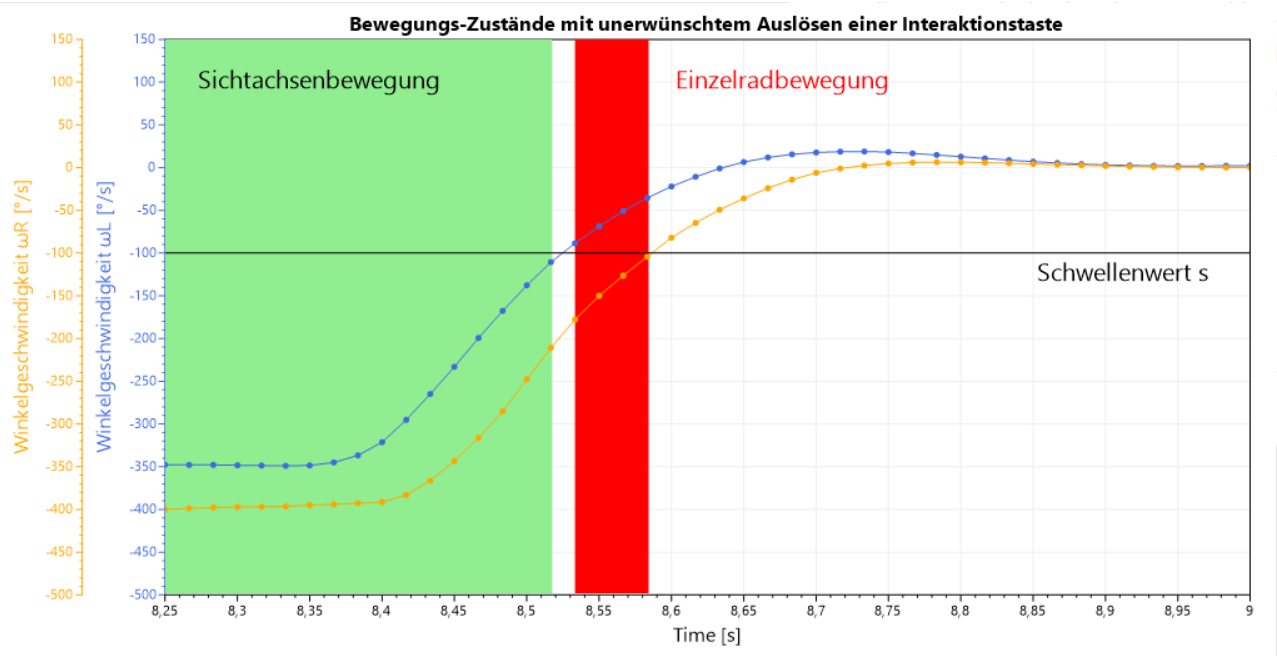
\includegraphics[width=0.75\textwidth]{1threshold.PNG}
    \caption{Bewegungs-Zustände mit unerwünschter \textit{Sichtachsenbewegung}}
    \label{fig:1_threshold}
\end{figure}

Dieses Problem lässt sich über das Einführen eines neuen \textit{Einzelradbewegung} Schwellenwertes beheben.
Wählt man für diesen einen geringeren Wert $s_1 = 25$ als für den Schwellwert für das Teilen des Wertebereichs $s_2$, entsteht eine Pufferzone.
Beim Beschleunigen überschreiten die Gyroskop-Werte zunächst nacheinander $s_1$. Anschließend überschreiten die Werte nacheinander $s_2$.
Solange beide Werte in der Pufferzone sind, kann weder eine \textit{Einzelradbewegung} noch eine \textit{Sichtachsenbewegung} detektiert werden (siehe Abbildung \ref{fig:2_threshold}).

\begin{figure}[h]
    \centering
    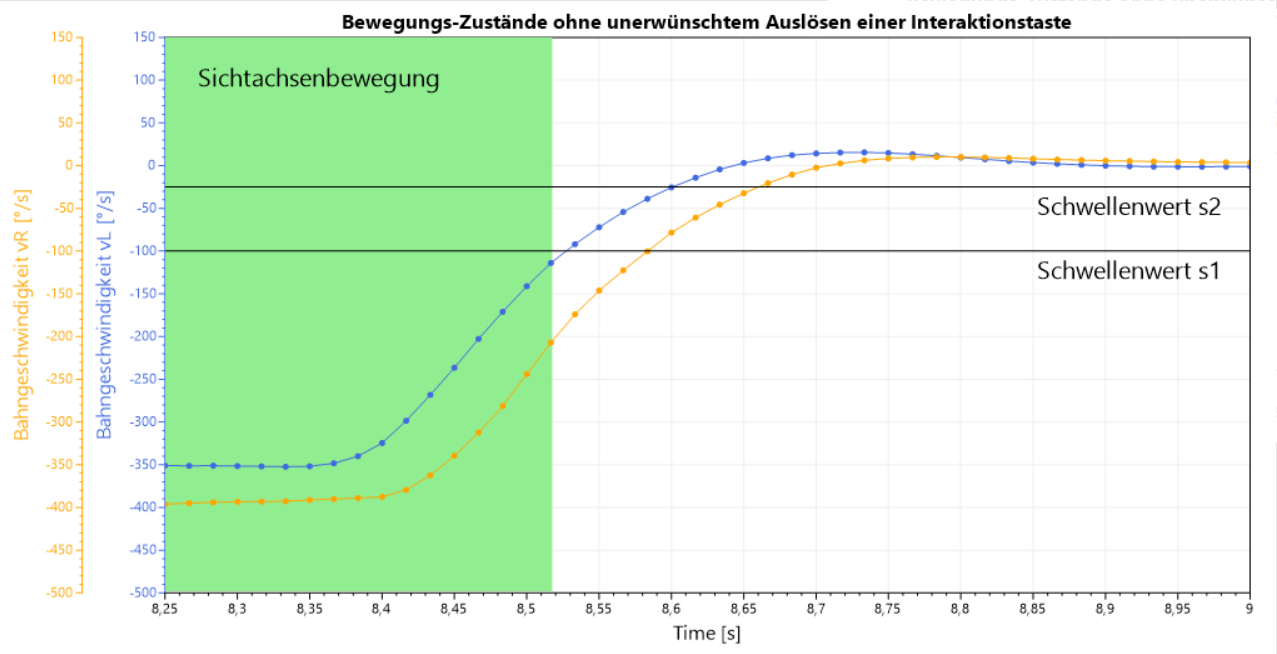
\includegraphics[width=0.75\textwidth]{2threshold.PNG}
    \caption{Bewegungs-Zustände ohne unerwünschter \textit{Sichtachsenbewegung}}
    \label{fig:2_threshold}
\end{figure}

Durch das Einführen der neuen Schwellenwerte müssen folgende Teilmengen-Bewegungszustände erweitert werden:

\textbf{\textit{Einzelradbewegung}}
\begin{align}
    ((|\omega_L| < s_1) \oplus (|\omega_R| < s_1)) \land ((|\omega_L| > s_2) \oplus (|\omega_R| > s_2))
\end{align}

\textbf{\textit{Sichtachsenbewegung}}
\begin{align}
    ((\omega_L > 0) \Leftrightarrow (\omega_R > 0)) \land ((|\omega_L| \geq s_2) \land (|\omega_R| \geq s_2))
\end{align}

\textbf{\textit{Neigen}}
\begin{align}
    ((\omega_L > 0) \Leftrightarrow (\omega_R > 0)) \land (|\omega_L| < s_2) \land (|\omega_R| < s_2)
\end{align}

\subsection{Unbeabsichtigtes Neigen beim Anfahren}
Beim Anfahren oder Bremsen (\textit{Sichtachsenbewegung}) wurde beobachtet, dass für ein kurzes Zeitintervall der Kamerawinkel unbeabsichtigt geneigt wird.
Ähnlich wie beim vorangegangenen Problem wird auch hier beim Übergang von einem Zustand zum Nächsten ein unerwünschter Zwischenzustand erreicht.
In diesem Fall gibt es beim Beschleunigen einen kurzes Zeitinterval in dem die Rollstuhl-Software im \textit{Neigen}-Zustand ist, da $|\omega_L|$ und $|\omega_R|$ beide unter dem Schwellenwert $s_2$ sind (siehe Abbildung \ref{fig:ohneAcc}).

\begin{figure}[h]
    \centering
    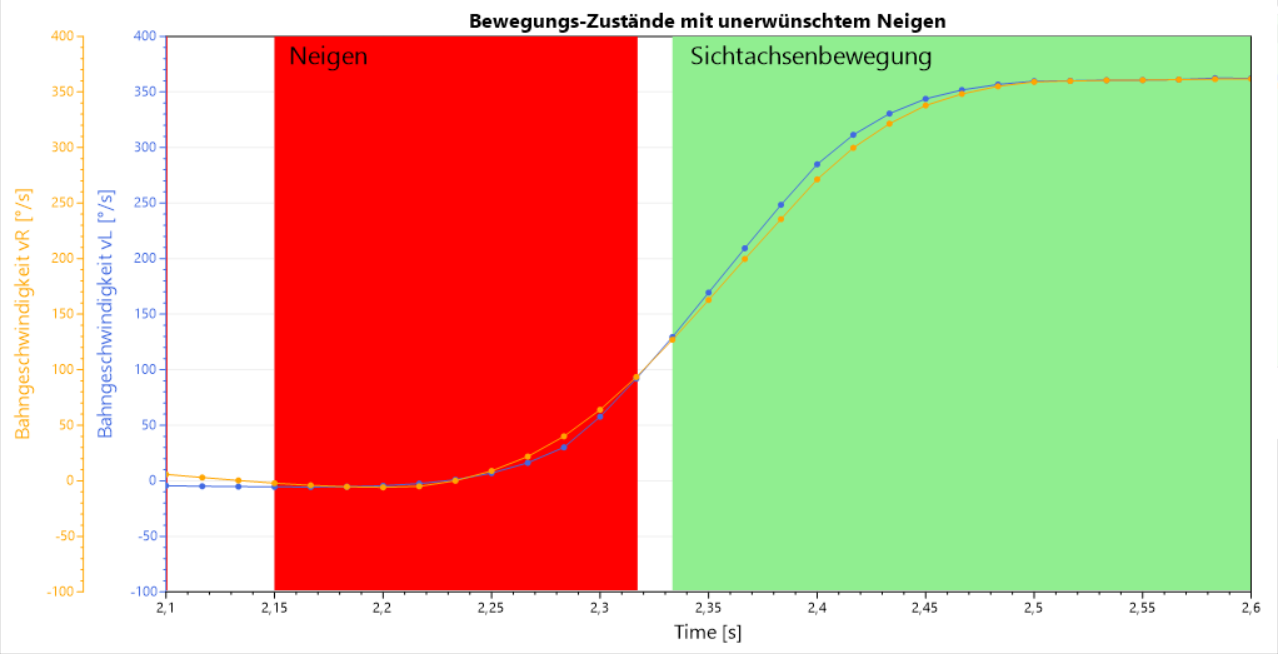
\includegraphics[width=0.75\textwidth]{ohneAcc.PNG}
    \caption{Bewegungs-Zustände mit unerwünschtem \textit{Neigen}}
    \label{fig:ohneAcc}
\end{figure}

Da die Fehldetektion immer dann auftritt, wenn sich die Geschwindigkeit der Räder ändert, ist der hier verwendete Lösungsansatz, die Bedingung des Neigungs-Zustandes zu erweitern.
In dieser wird nun auch abgefragt, ob die Summe der Änderungsraten $a$ der Gyroskope unter einem neuen Schwellenwert $s_3$ liegt.
Haben die Räder ihre Zielgeschwindigkeit erreicht, fällt die Änderungsrate unter $s_3$, sodass der nächste korrekte Zustand detektiert werden kann.
In den Tests hat sich $s_3 = 15$ als ein akzeptabler Wert herausgestellt, wie aus den Diagrammen abzulesen ist.
Für die Berechnung der Änderungsrate wird folgende Berechnung verwendet:
\begin{align}
    a = |(\omega_{L,[1]} - \omega_{L,[0]})| + |((\omega_{R,[1]} - \omega_{R,[0]})|
\end{align}

Die Bedingung des Teilmengen-Zustands \textit{Neigen} muss wie folgt ergänzt werden:

\textbf{\textit{Neigen}}
\begin{align}
    ((\omega_L > 0) \Leftrightarrow (\omega_R > 0)) \land (|\omega_L| < s_2) \land (|\omega_R| < s_2) \land (a < s_3)
\end{align}


\begin{figure}[h]
    \centering
    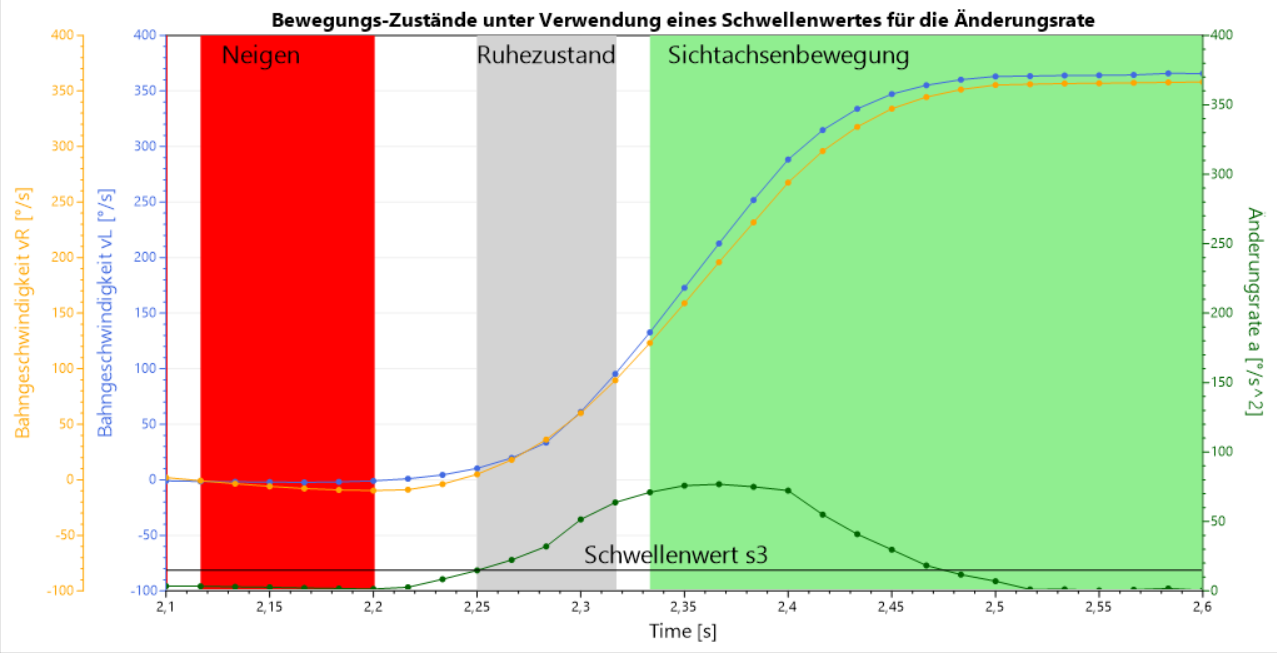
\includegraphics[width=0.75\textwidth]{mitAcc.PNG}
    \caption{Bewegungs-Zustände unter Verwendung eines Schwellenwertes für die Änderungsrate ohne unerwünschtem \textit{Neigen}}
    \label{fig:mitAcc}
\end{figure}

Aus der Abbildung \ref{fig:mitAcc} ist abzulesen, dass zwischen dem \textit{Sichtachsenbewegung}-Zustand und dem \textit{Neigen}-Zustand nun ein kurzer Ruhezustand existiert.
Diese Verzögerung bei der Fortbewegung ist vom Nutzer kaum bis gar nicht wahrnehmbar.
Im gezeigten Beispiel beträgt diese nur etwa 70ms.
Jedoch ist anzumerken, dass diese Methode vor allem bei ruckartigen Bewegungen funktioniert, da besonders dann die Änderungsrate schnell einen registrierbaren Ausschlag hat.
Verändert sich die Geschwindigkeit nicht schnell genug, kann es immer noch zu registrierbaren Neigungen kommen.


\chapter{Ausblick}
\chapter{Fazit}


%Literaturverzeichnis
\addcontentsline{toc}{chapter}{Literaturverzeichnis}
\printbibliography
% \bibliographystyle{acm}
% \bibliography{CitationDB}

%Abbildungsverzeichnis
\addcontentsline{toc}{chapter}{Abbildungsverzeichnis}
\listoffigures

%Abkürzungsverzeichnis
\addcontentsline{toc}{chapter}{Abkürzungsverzeichnis}
\chapter*{Abkürzungsverzeichnis}
\begin{acronym}
    \acro{pc}[PC]{Personal Computer}
    \acro{tcp}[TCP]{Transmission Control Protocol}
    \acro{udp}[UDP]{User Datagram Protocol}
    \acro{ip}[IP]{Internet Protocol}
    \acro{mac}[MAC]{Media Access Control}
    \acro{https}[HTTP(S)]{Hyper Text Transfer Protocol (Secure)}
    \acro{ui}[UI]{User Interface}
    \acro{gui}[GUI]{Graphical User Interface}
    \acro{ide}[IDE]{Integrated Development Environment}
    \acro{mems}[MEMS]{Micro Eelectro Mechanical Systems}
    \acro{rom}[ROM]{Read Only Memory}
    \acro{sram}[SRAM]{Static Random Access Memory}
    \acro{usb}[USB]{Universal Serial Bus}
    \acro{vr}[VR]{Virtual Reality}
\end{acronym}

\end{document}